\documentclass[12pt,]{article}
\usepackage{lmodern}
\usepackage{amssymb,amsmath}
\usepackage{ifxetex,ifluatex}
\usepackage{fixltx2e} % provides \textsubscript
\ifnum 0\ifxetex 1\fi\ifluatex 1\fi=0 % if pdftex
  \usepackage[T1]{fontenc}
  \usepackage[utf8]{inputenc}
\else % if luatex or xelatex
  \ifxetex
    \usepackage{mathspec}
  \else
    \usepackage{fontspec}
  \fi
  \defaultfontfeatures{Ligatures=TeX,Scale=MatchLowercase}
\fi
% use upquote if available, for straight quotes in verbatim environments
\IfFileExists{upquote.sty}{\usepackage{upquote}}{}
% use microtype if available
\IfFileExists{microtype.sty}{%
\usepackage{microtype}
\UseMicrotypeSet[protrusion]{basicmath} % disable protrusion for tt fonts
}{}
\usepackage[margin=1in]{geometry}
\usepackage{hyperref}
\hypersetup{unicode=true,
            pdftitle={Commodity Prices and the Business Cycle in resource-dependent Economies},
            pdfborder={0 0 0},
            breaklinks=true}
\urlstyle{same}  % don't use monospace font for urls
\usepackage{graphicx,grffile}
\makeatletter
\def\maxwidth{\ifdim\Gin@nat@width>\linewidth\linewidth\else\Gin@nat@width\fi}
\def\maxheight{\ifdim\Gin@nat@height>\textheight\textheight\else\Gin@nat@height\fi}
\makeatother
% Scale images if necessary, so that they will not overflow the page
% margins by default, and it is still possible to overwrite the defaults
% using explicit options in \includegraphics[width, height, ...]{}
\setkeys{Gin}{width=\maxwidth,height=\maxheight,keepaspectratio}
\IfFileExists{parskip.sty}{%
\usepackage{parskip}
}{% else
\setlength{\parindent}{0pt}
\setlength{\parskip}{6pt plus 2pt minus 1pt}
}
\setlength{\emergencystretch}{3em}  % prevent overfull lines
\providecommand{\tightlist}{%
  \setlength{\itemsep}{0pt}\setlength{\parskip}{0pt}}
\setcounter{secnumdepth}{0}
% Redefines (sub)paragraphs to behave more like sections
\ifx\paragraph\undefined\else
\let\oldparagraph\paragraph
\renewcommand{\paragraph}[1]{\oldparagraph{#1}\mbox{}}
\fi
\ifx\subparagraph\undefined\else
\let\oldsubparagraph\subparagraph
\renewcommand{\subparagraph}[1]{\oldsubparagraph{#1}\mbox{}}
\fi

%%% Use protect on footnotes to avoid problems with footnotes in titles
\let\rmarkdownfootnote\footnote%
\def\footnote{\protect\rmarkdownfootnote}

%%% Change title format to be more compact
\usepackage{titling}

% Create subtitle command for use in maketitle
\newcommand{\subtitle}[1]{
  \posttitle{
    \begin{center}\large#1\end{center}
    }
}

\setlength{\droptitle}{-2em}

  \title{Commodity Prices and the Business Cycle in resource-dependent Economies}
    \pretitle{\vspace{\droptitle}\centering\huge}
  \posttitle{\par}
    \author{Nikolas Kuschnig, Matthias Hagen \& Casper Engelen\\
WU Vienna, 5741 - Money, Credit \& Finance}
    \preauthor{\centering\large\emph}
  \postauthor{\par}
      \predate{\centering\large\emph}
  \postdate{\par}
    \date{08 August, 2018}

\usepackage{booktabs}
\usepackage{longtable}
\usepackage{array}
\usepackage{multirow}
\usepackage[table]{xcolor}
\usepackage{wrapfig}
\usepackage{float}
\usepackage{colortbl}
\usepackage{pdflscape}
\usepackage{tabu}
\usepackage{threeparttable}
\usepackage{threeparttablex}
\usepackage[normalem]{ulem}
\usepackage{makecell}

\usepackage{float}

\begin{document}
\maketitle
\begin{abstract}
This paper studies the impact of commodity price shocks in
resource-dependent economies, namely Australia, Chile, Norway and South
Africa. Principal Component Analysis is implemented as a way of reducing
the dimensionality of a multitude of available commodity prices and
inidces. Analysis of impulse responses in a recursively identified
structural Vector Autoregressive model is performed. We find
significant, differing responses to commodity price shocks for all
countries. Furthermore we find that the two selected principal
components lead to clearer, more significant impulse responses.
\end{abstract}

{
\setcounter{tocdepth}{3}
\tableofcontents
}
\newpage

\section{Introduction}\label{introduction}

The sources and drivers of business cycles have persistently been one of
the main subjects of macroeconomic research and will most likely remain
a staple of the discipline. The Vector Autoregressive (VAR) models
proposed by Sims (1980) as a method for policy analysis have shaped the
field ever since. A vast amount of literature focuses on the US business
cycle and considers various shocks, e.g.~due to technology, monetary
policy or commodity prices. However, the focus on the US, be it due to
data availability or importance of the country's economy, means that a
huge amount of information about business cycles has been left out -
other countries and their data have widely been neglected. On the other
hand, research combining business cycles and commodity prices has mainly
dealt with generic commodity price indices or specifically the oil
price.\\
This paper attempts to address both of these issues by considering a
multitude of commodity prices and indices for implementation in
structural VAR models spanning four resource-dependent economies
(Australia, Chile, Norway and South Africa). To our best knowledge this
approach has not been taken before, setting our work apart from the vast
literature we base it on. The theory is built upon the work of Gubler
and Hertweck (2013) on an extended set of business cycle shocks, that is
comprised of shocks via monetary policy, technology and commodity
prices. Gubler and Hertweck (2013) study the effect of commodity price
shocks in addition to the shocks presented by Altig et al. (2011) via a
structural VAR (SVAR) model of the US business cycle. They find
commodity price shocks to be an important source of fluctuation,
especially in regard to inflation (Gubler and Hertweck 2013, 20). Roch
(2017) focuses the analysis on terms-of-trade shocks in VAR models of
Chile, Colombia and Peru. The commodity price indices used are
country-specific and constructed from international prices and
country-level export data (Roch 2017, 6--7). Roch finds a ``substantial
impact {[}of terms-of-trade shocks{]} on fiscal aggregates'' (Roch 2017,
4), as well as a significant influence of fluctuations on key
macroeconomic variables. Further work on international business cycles
was done by Mallick and Sousa (2013), who evaluate the transmission of
monetary policy in five emerging market economies (Brazil, Russia,
India, China and South Africa). They use several types of VAR models and
uncover significant effects of a positive shock to commodity prices
(Mallick and Sousa 2013, 693).\\
We consider a structural VAR, identified via Cholesky decomposition and
interpret its impulse responses. Furthermore, we reduce the
dimensionality of multiple commodity price time series via Principal
Component Analysis (PCA). We find significant impacts of commodity
prices across models as well as evidence of the benefit of using PCA in
the form of substantially less impactful responses to non-transformed
commodity variables. This document is structured as follows: In section
2 the methodology regarding data, PCA and SVAR model are discussed. In
section 3 results are presented and outlined. Section 4 concludes.

\section{Methodology}\label{methodology}

\subsection{Data}\label{data}

In pursuit of a scientifically sound foundation to build further
analysis on, the initial concern of this paper was the definition and
selection of \emph{resource-dependent} countries. To avoid arbitrariness
this was done in a data-based manner. For this, World Bank data on
economic variables, resource rents and metal exports were utilised in
the creation of four indicators of resource-dependence. These are the
ratios of subsoil wealth to GDP, natural to total wealth, resource rents
to GDP and metal exports to total exports. Together with constraints on
size of the economy and ultimately data availability, these indicators
were used to single out Australia, Chile, Norway and South Africa for
our analysis. Furthermore, this group of countries was extended with
Germany and the United States - chosen for their size and excellent data
availability - as a kind of control group.\\
The major source for economic data was the OECD (2018), with time series
of quarterly GDP, trade, consumer prices, interest rates and many more.
While a wide array of data is readily available, length and frequency of
time series and comparability between countries posed some challenges.
E.g. vital time series on monetary policy rates were mostly gathered
from national central banks and - in the case of Australia and Norway -
had to be extended with short-term interbank rates. Data on unemployment
rates, exchange rates and other economic indicators were dropped due to
issues with heterogeneity and availability. Market data was gathered via
Bloomberg and Datastream and includes over forty commodity indices,
individual resource prices and equity indices. However, the bulk of
these time series only started in the 1990s, highlighting the dilemma of
longevity versus abundance of data. The temporal scope of the data was
adequate - more than 120 observations were avaialable for all countries
but Chile and Norway, which only featured 68 and 91 respectively. For a
more detailed overview of used data, its extent and its sources please
consult Tables 1, 2 and 5 in the appendix.\\
To achieve stationarity the variables, apart from interest rates, were
transformed. Three different approaches were up for consideration -
namely first-differences, log-differences and a Hodrick-Prescott filter.
Of these, log-differences performed best, with the exception of GDP,
which was filtered via an HP filter, and the principal components of the
resource data, where first-differences were applied.

\subsection{Vector Autoregression}\label{vector-autoregression}

\textbf{Vector Autoregressive} (VAR) models are a generalization of
univariate autoregressive (AR) models and are commonly resorted to as
tools for investigating the effects of economic shocks. They are based
on the notion of dynamic behaviour between the lags (\(p\)) of every
model variable. A VAR model of order \(p\) may be referred to as
\emph{VAR(p)} model and can be expressed as:
\[y_t = A_1 y_{t-1} + ... + A_p y_{t-p} + u_t\] Here \(y_t\) is a
\(K\)-dimensional vector of time series \(x_t\); \(A_{1, ..., p}\) are
\((K x K)\) matrices of coefficients and \(u_t\) is a \((K x 1)\) vector
of the linearly unpredictable component of \(y_t\). For shocks to have a
distinct economic interpretation one may recover structural shocks from
this reduced-form representation (Kilian and Lütkepohl 2017, 2)).
Consider: \[B_0 y_t = B_1 y_{t-1} + ... + B_p y_{t-p} + w_t\] With
\(B_{1, ..., p}\) as \((K x K)\) matrices of autoregressive slope
coefficients and \(w_t\) as a \((K x 1)\) vector of zero-mean structural
shocks, that is serially uncorrelated with a diagonal covariance matrix
\(\Sigma_w\) of full rank (Kilian and Lütkepohl 2017, 2). This
\emph{structural} form representation is obtained by pre-multiplying by
\(B_0^{-1}\), such that \(A_i = B_0^{-1} B_i\) and
\(u_t = B_0^{-1} w_t\). Thus, one has to estimate the matrix \(B_0\) (or
its inverse) to recover the structural model. Coming up with credible
restrictions for this matrix is known as the \emph{identification
problem}. Whilst there are diverse approaches to this problem, this
paper only takes the approach of recursive identification via Cholesky
decomposition. As described by Kilian and Lütkepohl (2017, 216), the
diagonal covariance matrix \(\Sigma\) can be expressed as the product of
two lower-triangular matrices \(PP’\), with \(B_0 = P\) as one possible
solution. However, in order to receive meaningful results one needs to
base the structure of \emph{P} on proper economic rationale. The fact
that \(P\) is a lower triangular matrix means that a certain causal
chain (higher variables react to fewer shocks contemporaneously) is
imposed on the data (Kilian and Lütkepohl 2017, 216) - a fact one has to
base the ordering of the model's variables on. Considering the variables
included in most of our models we order them as follows:

\begin{enumerate}
\def\labelenumi{\arabic{enumi}.}
\tightlist
\item
  Commodities
\item
  GDP
\item
  Inflation (CPI)
\item
  Exports
\item
  M3 Monetary Aggregate
\item
  Monetary Policy Rate
\item
  10Y Government Bond Yields
\item
  Equity Prices
\end{enumerate}

We attempt to categorise the variables in three broad categories: (1)
variables that react to monetary policy shocks with a lag; (2) the
monetary policy rate; and (3) variables that adjust contemporaneously to
a monetary policy shock. We limit the third group to fixed income and
equity prices, which is broadly based on the notion of efficient markets
(Malkiel and Fama 1970). In line with previous work (e.g. Mallick and
Sousa (2013)) we place the GDP, inflation and other macroeconomic
variables towards the top. Commodity prices are placed on top, according
to Kilian and Vega (2011), who formally test different identifying
assumptions regarding oil prices. They find no compelling evidence of
short-term feedback, i.e.~at the monthly horizon, to macroeconomic news,
thus lending support to theoretical models based on this hypothesis
(Kilian and Vega 2011, 16--17). The chosen lag-lengths were based on the
\emph{Akaike Information Criterion} and resulting impulse responses;
they ultimately ended up at one for each model.

\subsection{Variable Selection}\label{variable-selection}

\textbf{Principal component Analysis} (PCA) can be used to reduce the
dimensionality of a dataset with many interrelated variables, whilst
also conserving as much of the variation present in the data set as
possible (Abdi and Williams 2010; Stock and Watson 2002). To achieve
this, PCA focuses on variances, without neglecting covariances and
correlations. Due to its versatile nature, PCA is one of the most widely
utilised multivariate statistical techniques and has found application
in a multitude of scientific disciplines (Abdi and Williams 2010). The
variables created in the PCA process can be useful for forecasting in
macroeconomic analysis (Stock and Watson 2002; Favero, Marcellino, and
Neglia 2005), where many different variables and time series are
generally available. Since we want to model the effect of a plethora of
commodity prices on business cycles within a VAR framework - notorious
for its curse of dimensionality - it is beneficial to reduce the number
of variables that are used in the estimation. VAR models benefit greatly
from being set up parsimoniously and the reduction of dimensionality
that can be achieved via PCA should lead to better results.\\
Regarding the methodology consider the vector \(x\) with \(p\) random
variables, where we are interested in the variances of the random
variables and the structure of covariances and correlations between
them. If the number of random variables is high, or the structure is
complex, it is often helpful to look for few derived variables, that
preserve the information of the variances, correlations and covariances,
instead of examining them directly (Jolliffe 2011). When using PCA these
new, derived variables are called the principal components. They are
uncorrelated and retain most of the variation present in the entire
dataset (Jolliffe 2011). Initially, PCA finds a linear function
\(\alpha_1' x\) of the elements of \(x\) while maximizing variance,
where \(\alpha_1'\) is a vector of \emph{p} constants. Hence:
\[\alpha_1’x = \alpha_{11} x_1 + \alpha_{12} x_2 + ... + \alpha_{1p} x_p = \sum_{j=1}^p \alpha_{1j} x_j\]
Next, PCA looks for a linear function \(\alpha_2' x\) that is
uncorrelated with \(\alpha_1'\) while also having maximum variance, and
so on, so that the \(k\)-th stage yields the linear function
\(\alpha_k’ x\), again uncorrelated with all linear functions
\(\alpha_1' x, ..., \alpha_{k-1}' x\) and with maximum variance. Up to
\(p\) principal components can be distinguished, although the aim is to
find an amount \(m\), such that \(m << p\), thus reducing the
dimensionality of the dataset. The values of these resulting variables
are called \emph{factor scores}, and form their own time series (Abdi
and Williams 2010; Stock and Watson 2002).\\
For PCA to be successful, the considered variables should be correlated,
but not perfectly so, since this would hinder a reduction in the
dimensionality. To evaluate whether PCA can be used to reduce
dimensionality one may use the \emph{KMO-Criterion} and the p-value of
\emph{Bartlett's Test of Sphericity}. Afterwards, a balance has to be
struck between providing a sufficient amount of observations to the VAR
model, whilst also capturing as much information as possible from the
commodity markets. There are several established criteria for handling
this tradeoff, although the exact cut-off points are somewhat subjective
(Abdi and Williams 2010). The number of principal components is
determined via the components' eigenvalues, which are equal to the sum
of squared factor scores. The Kaiser Criterion (Kaiser 1961) suggests a
cut-off eigenvalue of one and is chosen due to its prevalence and
sufficient reduction of dimensionality.

Furthermore, \textbf{Bayesian Model Averaging} (BMA) is used as an
additional way of assessing the model's structure. In short, BMA deals
with the question of which independent variables to include in a model.
Conceptionally this would be done by obtaining the results of every
feasible model and averaging them (Koop 2003, 266). In practice it
swiftly becomes an impossible task, as the number of possible
combinations may very well be enormous. However, since the models
considered here do not exceed nine variables, we are able to enumerate
the entire model space using the R package \emph{BMS} by Zeugner,
Feldkircher, and others (2015).

\section{Results}\label{results}

\subsection{Variable Structure}\label{variable-structure}

For the optimal choice of dataset to be handled with PCA, several
starting points of the commodity time series were considered (see
Appendix, Table 4). Ultimately the second quarter of 1979 was selected,
as it yielded the strongest test-statistics with regards to the
possibility of using PCA, while also being covered by a sizeable amount
of the available time series (see Appendix, Table 5). A KMO-Criterion of
0.803 and a highly significant p-value of Bartlett's Test of Sphericity
indicate the suitability of PCA. The \emph{Kaiser Criterion} yields two
components that add a satisfactory amount of information to the model.
The components have eigenvalues of 7.79 and 2.68 (see Appendix, Table 6)
which are both well above the cut-off. Additionally, the components
capture 60 and 21 percent of the sample variance - which is considered
sensible (Jolliffe, 2011). Based on the resulting factor loadings one
can distinguish between the variables in each component. Whilst the
first component comprises time series of precious metals, agriculture \&
livestock and a generic commodity index, the second one contains
industrial metals. Thus we will refer to them as \emph{Commodities} and
\emph{Industrial Metals} (labelled \emph{comm} and \emph{industr}).

The iteratively computed posterior inclusion probabilities (PIPs)
provide an interesting overview of the data (see Appendix, Figures 6 \&
7), but should be interpreted with care. In the case of Australia the
commodities' principal components display very low PIPs, a picture that
holds for all variables. The Chilean data however, appear to be rather
interconnected. The commodity variables show decent inclusion in models
explaining the monetary policy rate, the monetary aggregate, exports and
even GDP. The Norwegian PIPs are generally rather low, although the
commodity components turn out relatively high, with high inclusion when
explaining GDP and decent values for equity prices. For South Africa the
PIPs turn out slightly higher - the principal components show up when
explaining the monetary policy rate, inflation and GDP. Based on these
results we would expect higher impacts of the commodity components for
Chile and South Africa, while one could presume the lower interplay of
variables for Australia and Norway to lead to less convoluted models.

\subsection{Impulse Responses}\label{impulse-responses}

The impulse responses, as pictured in Figures 1 and 2 (as well as
Appendix, Figures 3, 4 \& 5) show us the reaction of the model's
variables to specific shocks. The solid black line corresponds to the
mean response; the dark- and light-gray areas cover 25-75 percent and
16-84 percent posterior confidence intervals among the 10,000
iterations.

\begin{figure}
\centering
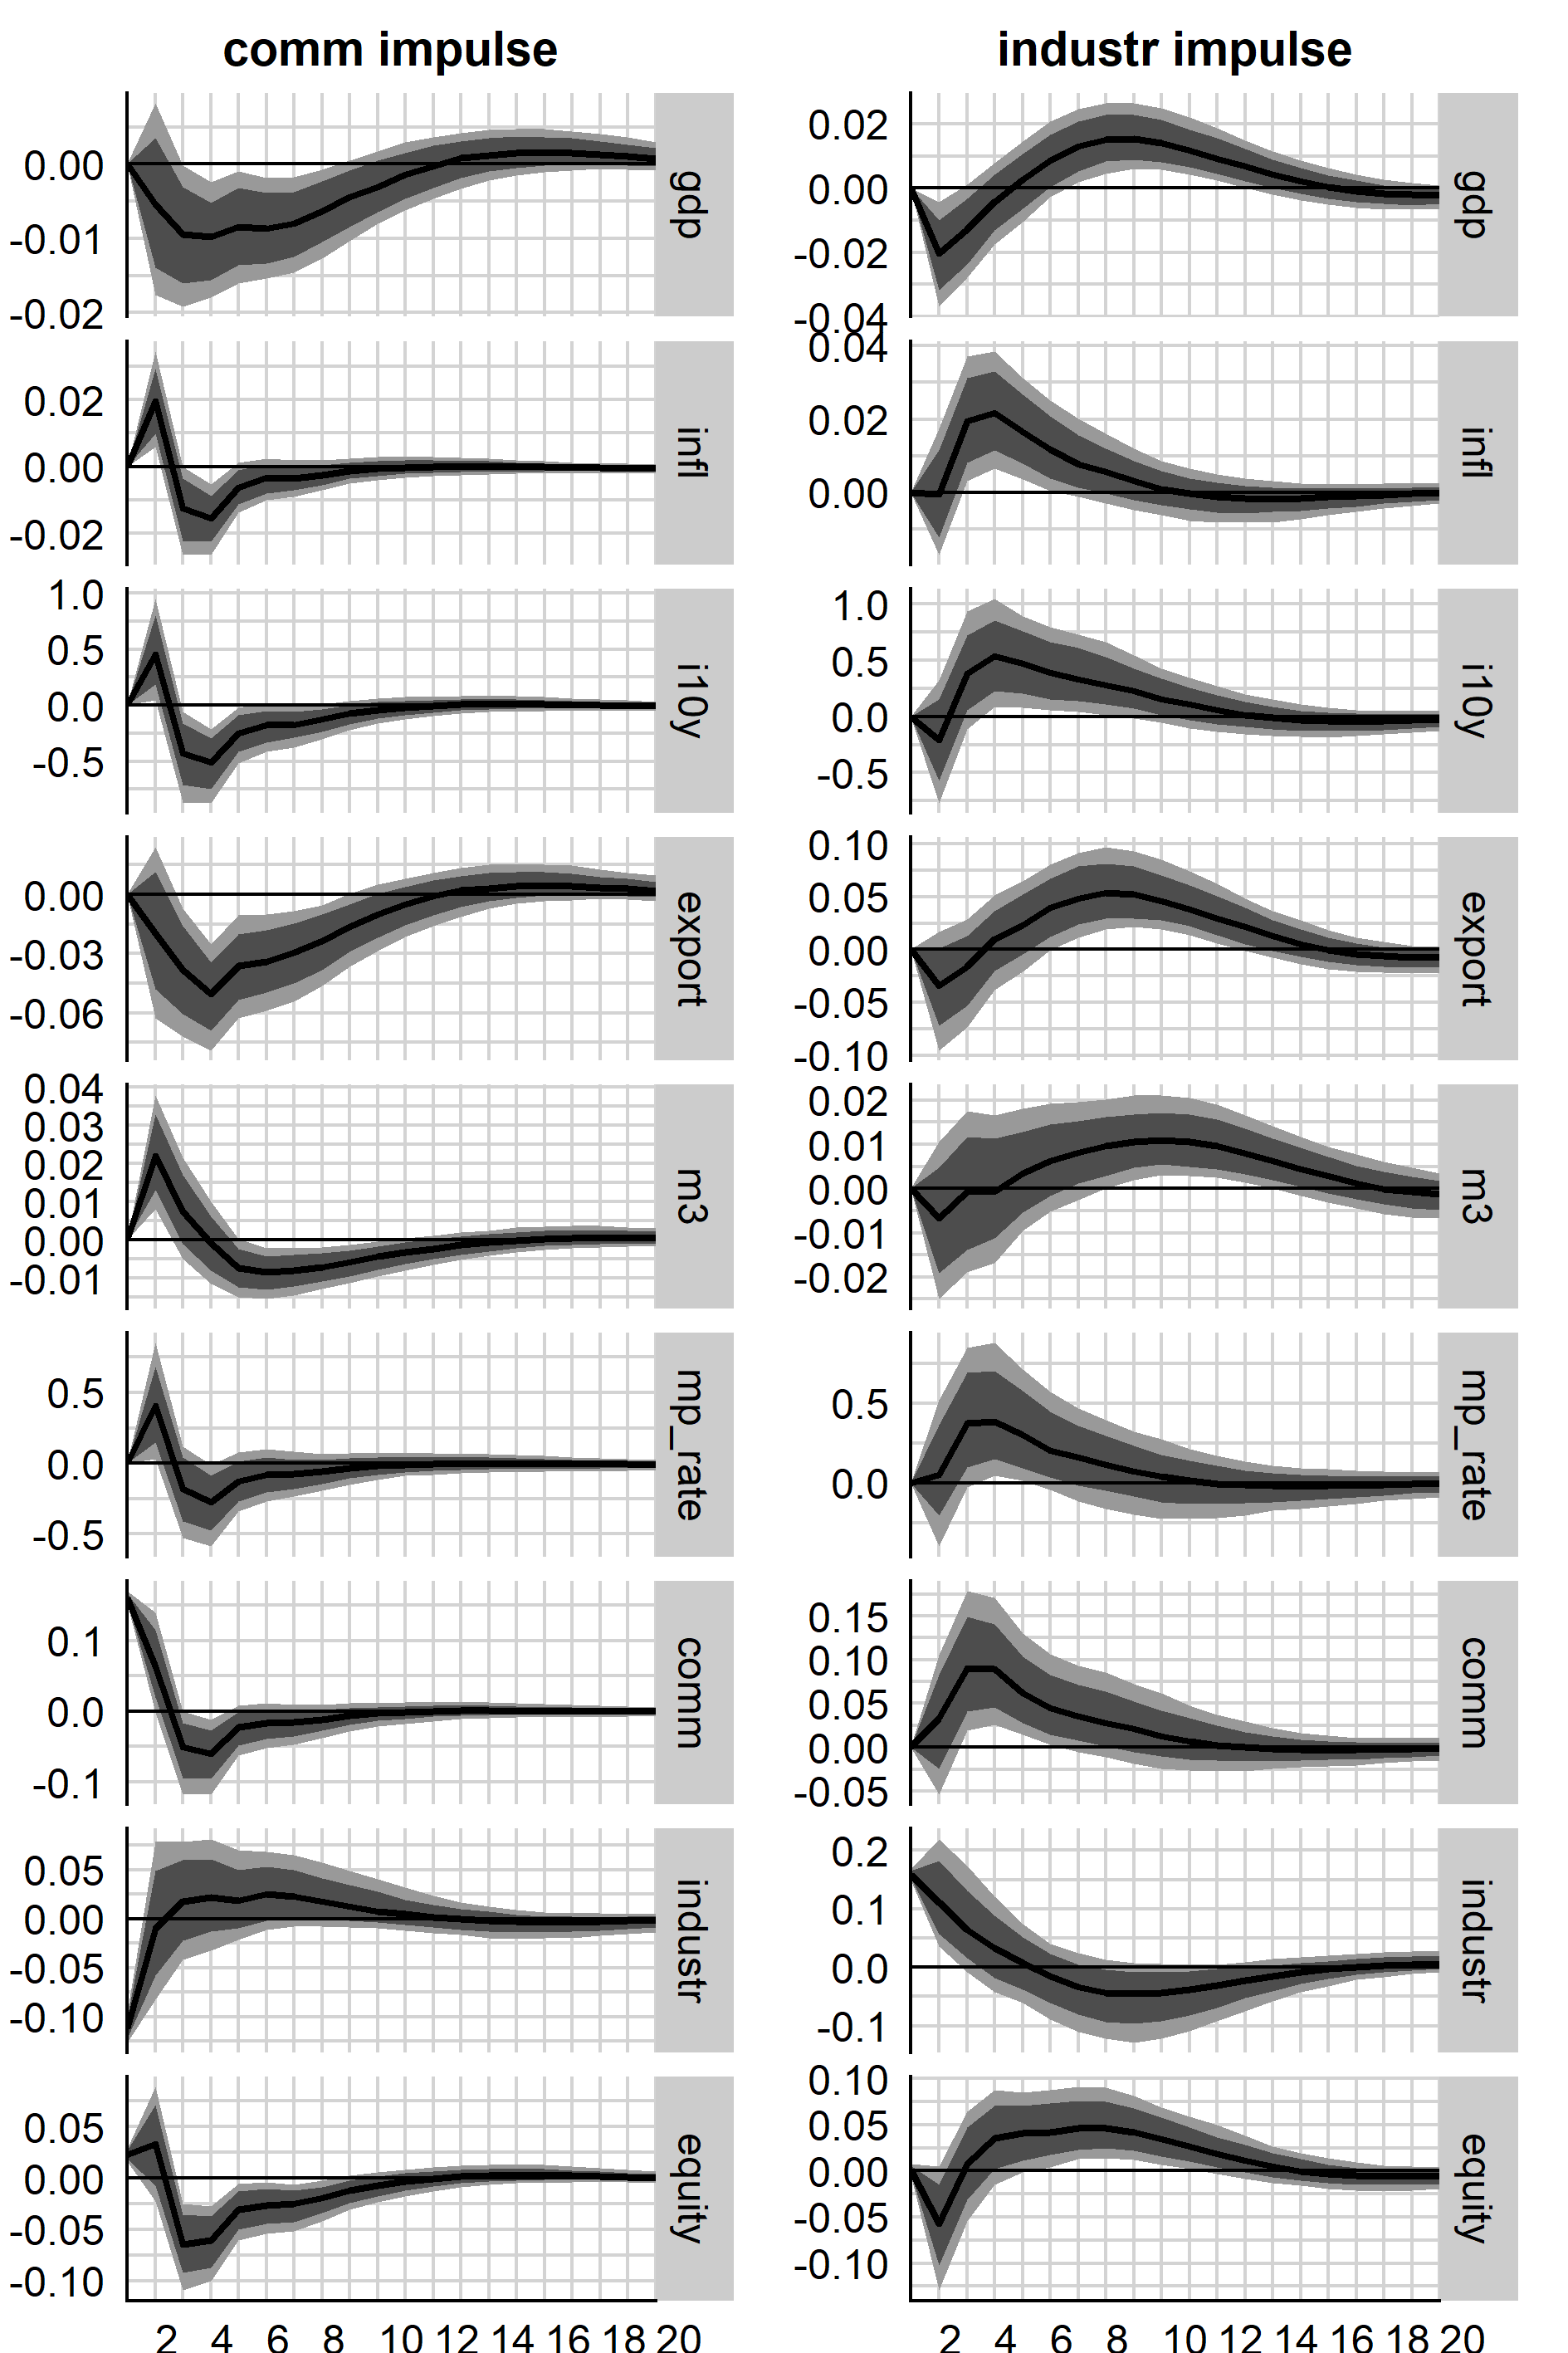
\includegraphics[width=0.50000\textwidth]{img/irf_short_ZAF.png}
\caption{Commodity Impulse Responses, South Africa}
\end{figure}

\begin{figure}
\centering
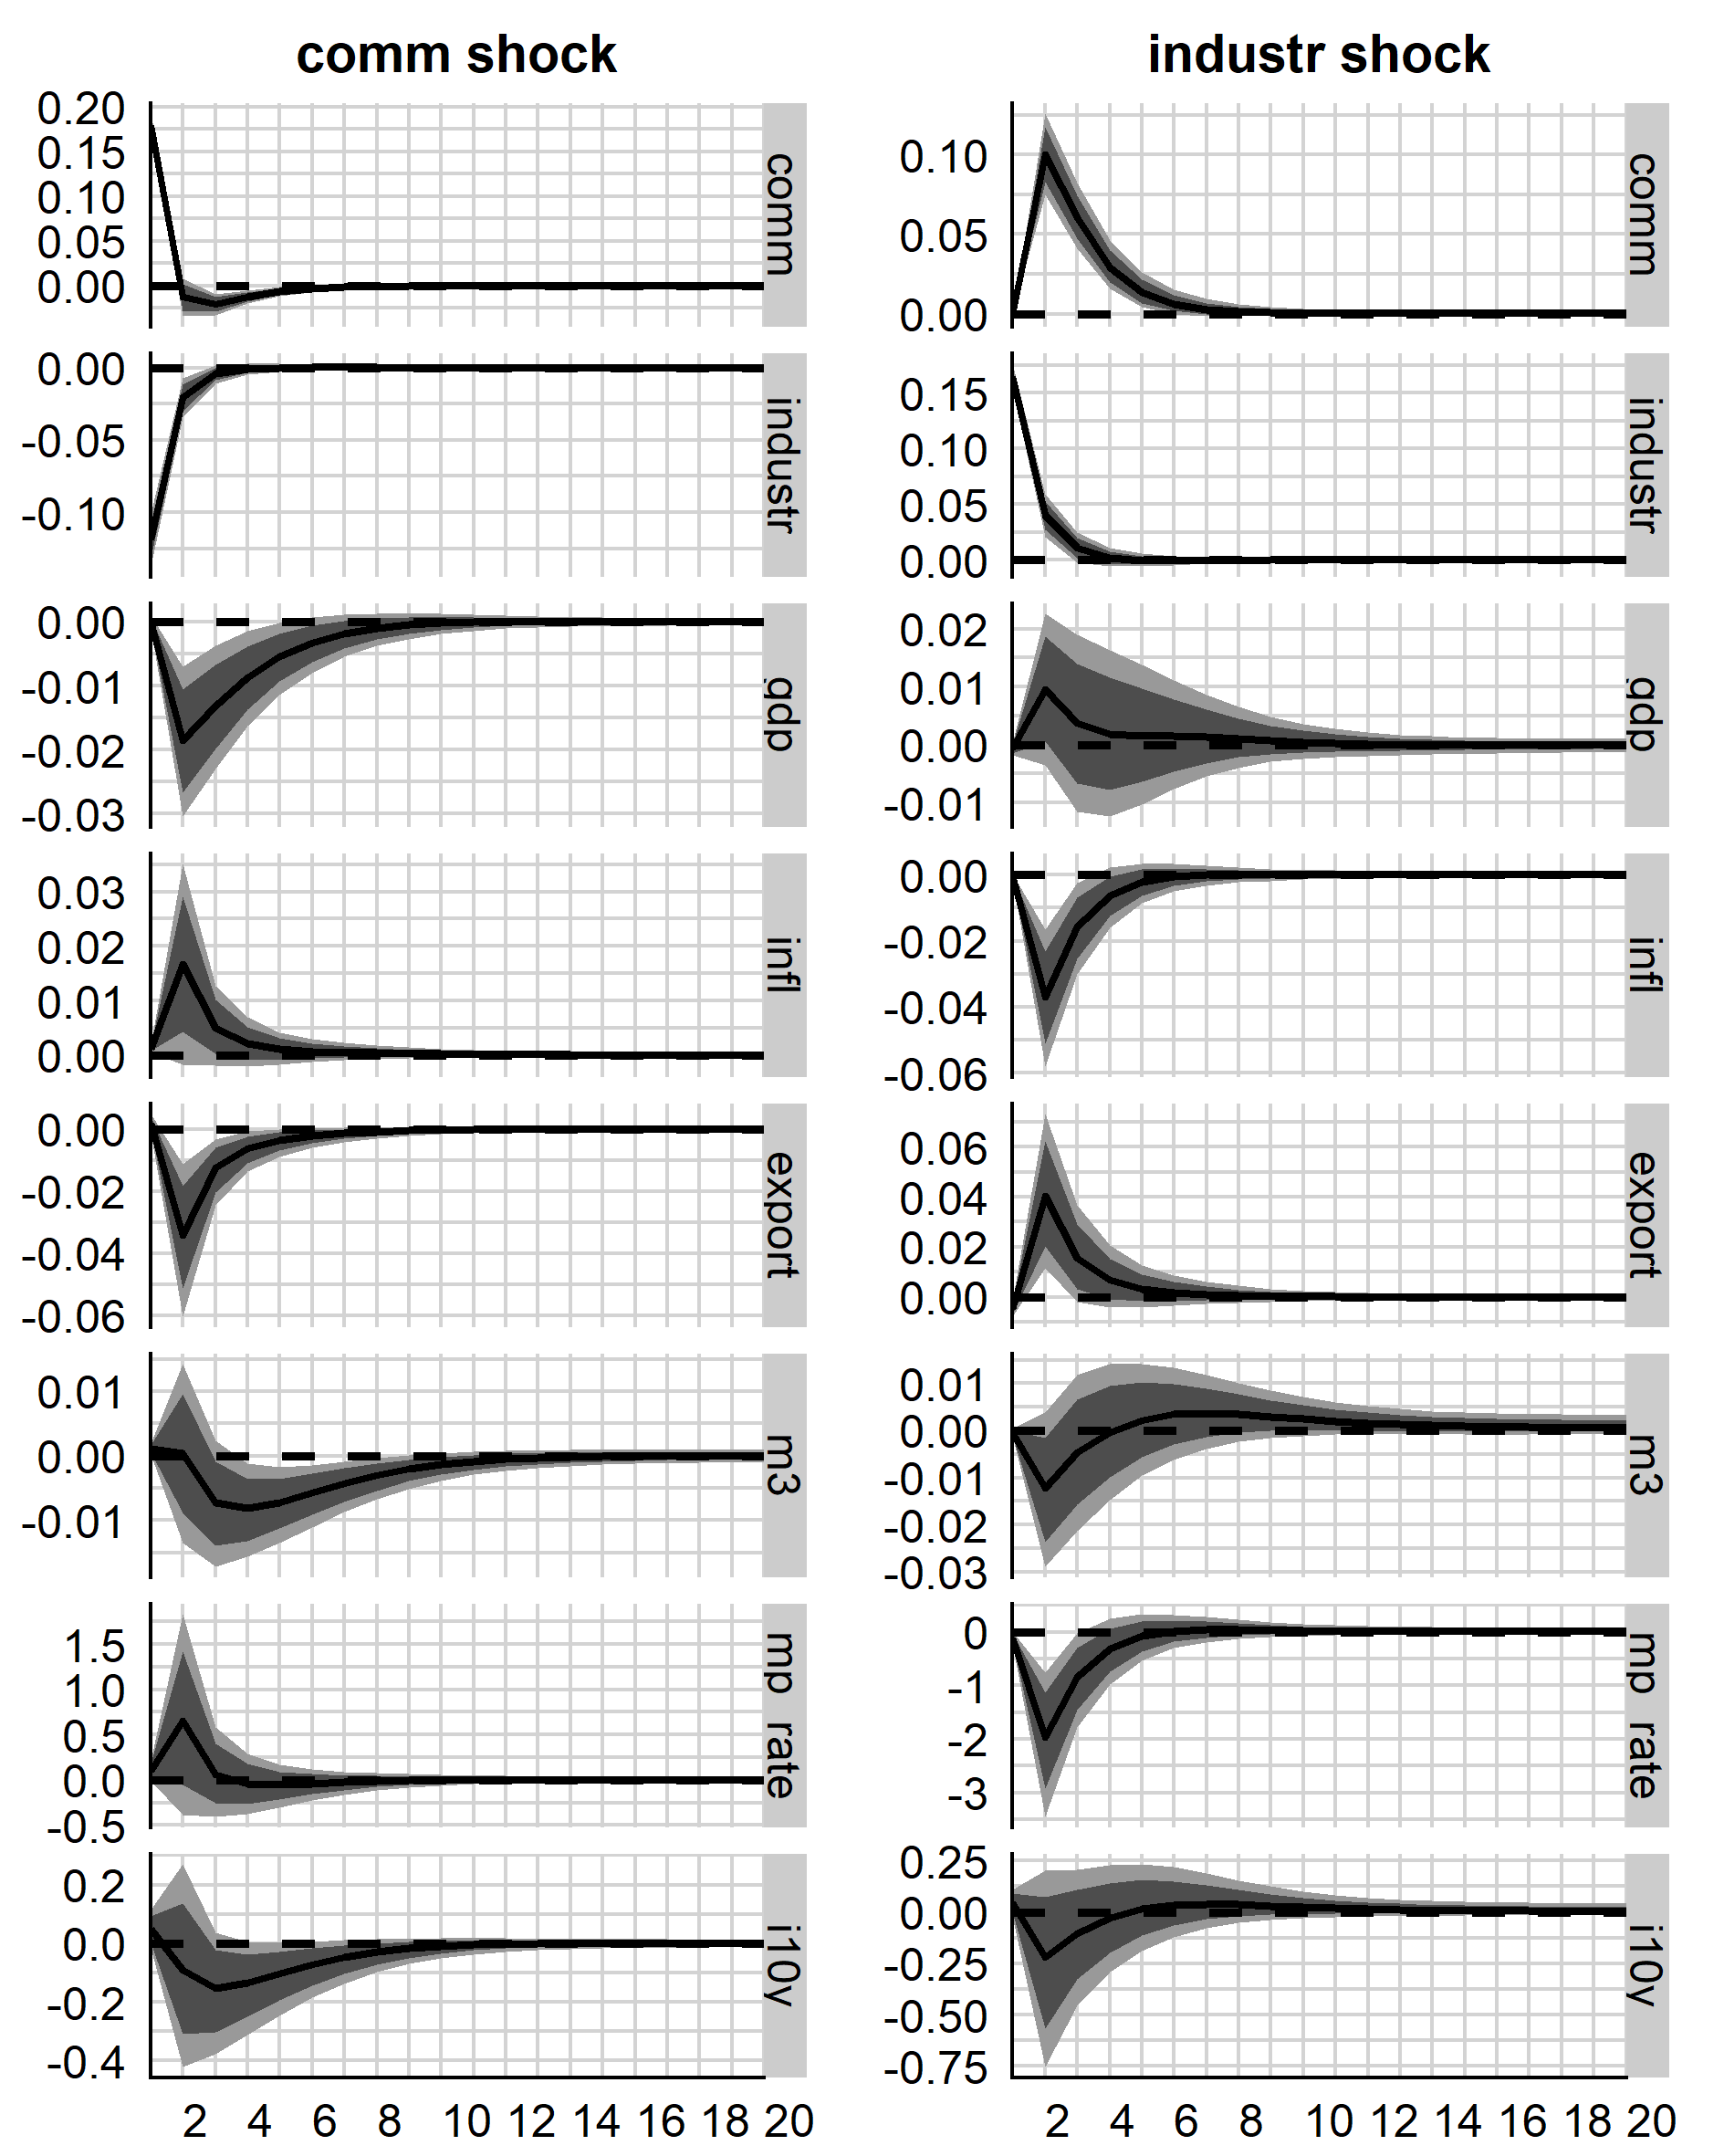
\includegraphics[width=0.50000\textwidth]{img/irf_short_AUS.png}
\caption{Commodity Impulse Responses, Australia}
\end{figure}

The obtained impulse responses reveal a prominent reciprocity between
the principal components of commodity prices and key macroeconomic
indicators. Beside commodities technology shocks roughly turn out as
expected, and do so rather significantly. In the cases of inflation and
monetary aggregates the responses may be pronounced, but tend to
dissipate very quickly. The picture of monetary policy shocks is rather
diverse - responses vary across countries in direction, significance and
persistence. A shock to the first principal component (labelled
\emph{comm}) impacted GDP negatively in all countries, but Chile.
Similar things held for inflation, which received a boost in most
models, except for Chile's, where it fell, and Norway's where it fell
insignificantly. The impacts on export were rather negative for
resource-dependent economies, but positive on the control-group of
Germany and the US. The monetary policy rate reacted in an expansionary
matter for Australia and the US, but insignificantly or contractionarily
for the other countries. In German and South African models we can also
observe a short, but significant jump in equity prices as a reaction to
a shock on this first principal component. The second principal
component (labelled \emph{industr}) did not affect GDP as consistently;
although, the initial effect was positive in all models, but Chile's. In
the control group this positive GDP response even increased for a while
and only faded after a considerable amount of time. In the
resource-dependent countries the responses peaked rather early and
subsequently tended to insignificance. Meanwhile, the effects on
inflation, bond-yields, monetary aggregates and the monetary policy
rates differed between countries, but turned out extremely similar in
each country itself. Exports jumped significantly for Australia and
South Africa, whereas they fell in the models of Germany and the US,
only to rebound to a small but significant increase after about four to
six quarters. Curiously the shock also had a significant, positive
effect on South African equity prices.\\
Another set of models with country-specific commodities instead of
principal components was estimated for comparison. These include
industrial metals, agriculture and livestock, gold, copper, energy and
precious metals (see Appendix, Table 3). The resulting impulse responses
were largely comparable, but the impacts and responses of commodity
variables turned out rather insignificant. Ultimately this approach
yielded less convincing results than one that simply used a single
commodity price index. We interpret this as evidence for our approach of
using principal components, as it combines the advantage of both methods
- the use of all available data, including rather country-specific time
series, and the impactfulness of using few, but significant variables.

\section{Discussion}\label{discussion}

This paper deals with the impact of commodity price shocks on economic
variables in four resource-dependent countries. Principal Component
Analysis was used to compress information on multiple commodity time
series; the resulting principal components were then added to a
structural Vector Autoregressive model alongside several variables of
interest. Identification was conducted recursively on the premise that
commodity prices do not react to macroeconomic news in the short-term -
an assumption based on Kilian and Vega (2011). The resulting impulse
response functions showed varying, significant responses of
macroeconomic indicators to commodity price shocks across the countries
examined. Comparison with models with either a standard commodity index
or country-specific commodities yielded less - if at all - pronounced
impulse responses, which might suggest the advantageousness of our
approach.\\
Considering the interesting results and the modular nature of the
analysis manifold extensions to this paper are conceivable. For one, an
expansion of the data and/or the countries surveyed would present
itself. The econometric model employed might benefit from changes in
identification - be it through different ordering or a different scheme
altogether. Also analysis itself would be comfortably expandable via
historical or variance decomposition. Furthermore, one could apply a
global VAR or various Bayesian methods, such as priors (possibly with
hyperparameters) and/or stochastic volatility.

\newpage

\section{Literature}\label{literature}

\hypertarget{refs}{}
\hypertarget{ref-abdi2010principal}{}
Abdi, Hervé, and Lynne J Williams. 2010. ``Principal Component
Analysis.'' \emph{Wiley Interdisciplinary Reviews: Computational
Statistics} 2 (4). Wiley Online Library: 433--59.

\hypertarget{ref-altig2011firm}{}
Altig, David, Lawrence J Christiano, Martin Eichenbaum, and Jesper
Linde. 2011. ``Firm-Specific Capital, Nominal Rigidities and the
Business Cycle.'' \emph{Review of Economic Dynamics} 14 (2). Elsevier:
225--47.

\hypertarget{ref-favero2005principal}{}
Favero, Carlo A, Massimiliano Marcellino, and Francesca Neglia. 2005.
``Principal Components at Work: The Empirical Analysis of Monetary
Policy with Large Data Sets.'' \emph{Journal of Applied Econometrics} 20
(5). Wiley Online Library: 603--20.

\hypertarget{ref-gubler2013commodity}{}
Gubler, Matthias, and Matthias S Hertweck. 2013. ``Commodity Price
Shocks and the Business Cycle: Structural Evidence for the Us.''
\emph{Journal of International Money and Finance} 37. Elsevier: 324--52.

\hypertarget{ref-jolliffe2011principal}{}
Jolliffe, Ian. 2011. ``Principal Component Analysis.'' In
\emph{International Encyclopedia of Statistical Science}, 1094--6.
Springer.

\hypertarget{ref-kaiser1961note}{}
Kaiser, Henry F. 1961. ``A Note on Guttman's Lower Bound for the Number
of Common Factors.'' \emph{British Journal of Statistical Psychology} 14
(1). Wiley Online Library: 1--2.

\hypertarget{ref-kilian2017structural}{}
Kilian, Lutz, and Helmut Lütkepohl. 2017. \emph{Structural Vector
Autoregressive Analysis}. Cambridge University Press.

\hypertarget{ref-kilian2011energy}{}
Kilian, Lutz, and Clara Vega. 2011. ``Do Energy Prices Respond to Us
Macroeconomic News? A Test of the Hypothesis of Predetermined Energy
Prices.'' \emph{Review of Economics and Statistics} 93 (2). MIT Press:
660--71.

\hypertarget{ref-koop2003bayesian}{}
Koop, G. 2003. \emph{Bayesian Econometrics}. Wiley.

\hypertarget{ref-malkiel1970efficient}{}
Malkiel, Burton G, and Eugene F Fama. 1970. ``Efficient Capital Markets:
A Review of Theory and Empirical Work.'' \emph{The Journal of Finance}
25 (2). Wiley Online Library: 383--417.

\hypertarget{ref-mallick2013commodity}{}
Mallick, Sushanta K, and Ricardo M Sousa. 2013. ``Commodity Prices,
Inflationary Pressures, and Monetary Policy: Evidence from Brics
Economies.'' \emph{Open Economies Review} 24 (4). Springer: 677--94.

\hypertarget{ref-oecd2018indicators}{}
OECD. 2018. \emph{Main Economic Indicators, Volume 2018 Issue 7}.
doi:\href{https://doi.org/https://doi.org/10.1787/mei-v2018-7-en}{https://doi.org/10.1787/mei-v2018-7-en}.

\hypertarget{ref-roch2017adjustment}{}
Roch, Francisco. 2017. \emph{The Adjustment to Commodity Price Shocks in
Chile, Colombia, and Peru}. International Monetary Fund.

\hypertarget{ref-sims1980macroeconomics}{}
Sims, Christopher A. 1980. ``Macroeconomics and Reality.''
\emph{Econometrica: Journal of the Econometric Society}. JSTOR, 1--48.

\hypertarget{ref-stock2002forecasting}{}
Stock, James H, and Mark W Watson. 2002. ``Forecasting Using Principal
Components from a Large Number of Predictors.'' \emph{Journal of the
American Statistical Association} 97 (460). Taylor \& Francis: 1167--79.

\hypertarget{ref-zeugner2015bayesian}{}
Zeugner, Stefan, Martin Feldkircher, and others. 2015. ``Bayesian Model
Averaging Employing Fixed and Flexible Priors: The Bms Package for R.''
\emph{Journal of Statistical Software} 68 (4). Foundation for Open
Access Statistics: 1--37.

\section{Appendix}\label{appendix}

\begin{table}[!h]

\caption{\label{tab:unnamed-chunk-2}Data used in the VAR model}
\centering
\begin{tabular}[t]{l|l|l|l|l|l|l}
\hline
- & AUS & CHL & DEU & NOR & USA & ZAF\\
\hline
Commodities & 1979Q4- & 1979Q4- & 1979Q4- & 1979Q4- & 1979Q4- & 1979Q4-\\
\hline
GDP & 1977Q2- & 1995Q2- & 1960Q1- & 1983Q4- & 1960Q1- & 1973Q2-\\
\hline
Inflation (CPI) & 1977Q2- & 1978Q2- & 1960Q1- & 1983Q4- & 1960Q1- & 1973Q2-\\
\hline
Exports & 1977Q2- & 1995Q2- & 1960Q1- & 1983Q4- & 1960Q1- & 1973Q2-\\
\hline
M3 & 1977Q2- & 1986Q2 & 1960Q1- ** & 1983Q4- & 1960Q1- & 1973Q2-\\
\hline
Monetary Policy & 1977Q2- * & 1995Q2- & 1960Q2- & 1983Q4- * & 1960Q1- & 1973Q2-\\
\hline
10Y Bond Yields & 1977Q2- & 2004Q4- *** & 1960Q1- & 1984Q4- & 1960Q1- & 1973Q2-\\
\hline
Equity Indices & 1999Q2- *** & 1987Q3- & 1960Q2- & 1987Q3- & 1964Q2- & 1973Q2-\\
\hline
\multicolumn{7}{l}{\textit{Note: }}\\
\multicolumn{7}{l}{* Gaps filled with short-term (3M) Interbank rates}\\
\multicolumn{7}{l}{** M2 used due to availability}\\
\multicolumn{7}{l}{*** Variable dropped due to availability}\\
\end{tabular}
\end{table}

\begin{table}[!h]

\caption{\label{tab:unnamed-chunk-3}Data used in the VAR model}
\centering
\begin{tabular}[t]{l|l|l|l|l}
\hline
- & Source & Subject & Measure & Frequency\\
\hline
Commodities & Bloomberg & - & - & M\\
\hline
GDP & OECD & B1\_GE & CPCARSA & Q\\
\hline
Inflation (CPI) & OECD & CPALTT01 & IXOB & Q\\
\hline
Exports & OECD & P7 & CPCARSA & Q\\
\hline
M3 & OECD, FRED & MABMM301 & IXOBSA & Q\\
\hline
Monetary Policy & Central Banks, FRED & - & - & -\\
\hline
10Y Bond Yields & OECD & IRLTLT01 & - & Q\\
\hline
Equity Indices & Datastream & - & - & M\\
\hline
\end{tabular}
\end{table}

\begin{table}[!h]

\caption{\label{tab:unnamed-chunk-4}Alternative, country-specific commodity variables}
\centering
\begin{tabular}[t]{l|l|l|l|l}
\hline
Country & Australia & Chile & Norway & South Africa\\
\hline
Commodity 1 & Industrial Metals & Copper & Energy & Precious Metals\\
\hline
Commodity 2 & Agriculture \& Livestock & Gold & - & -\\
\hline
\end{tabular}
\end{table}

\begin{figure}
\centering
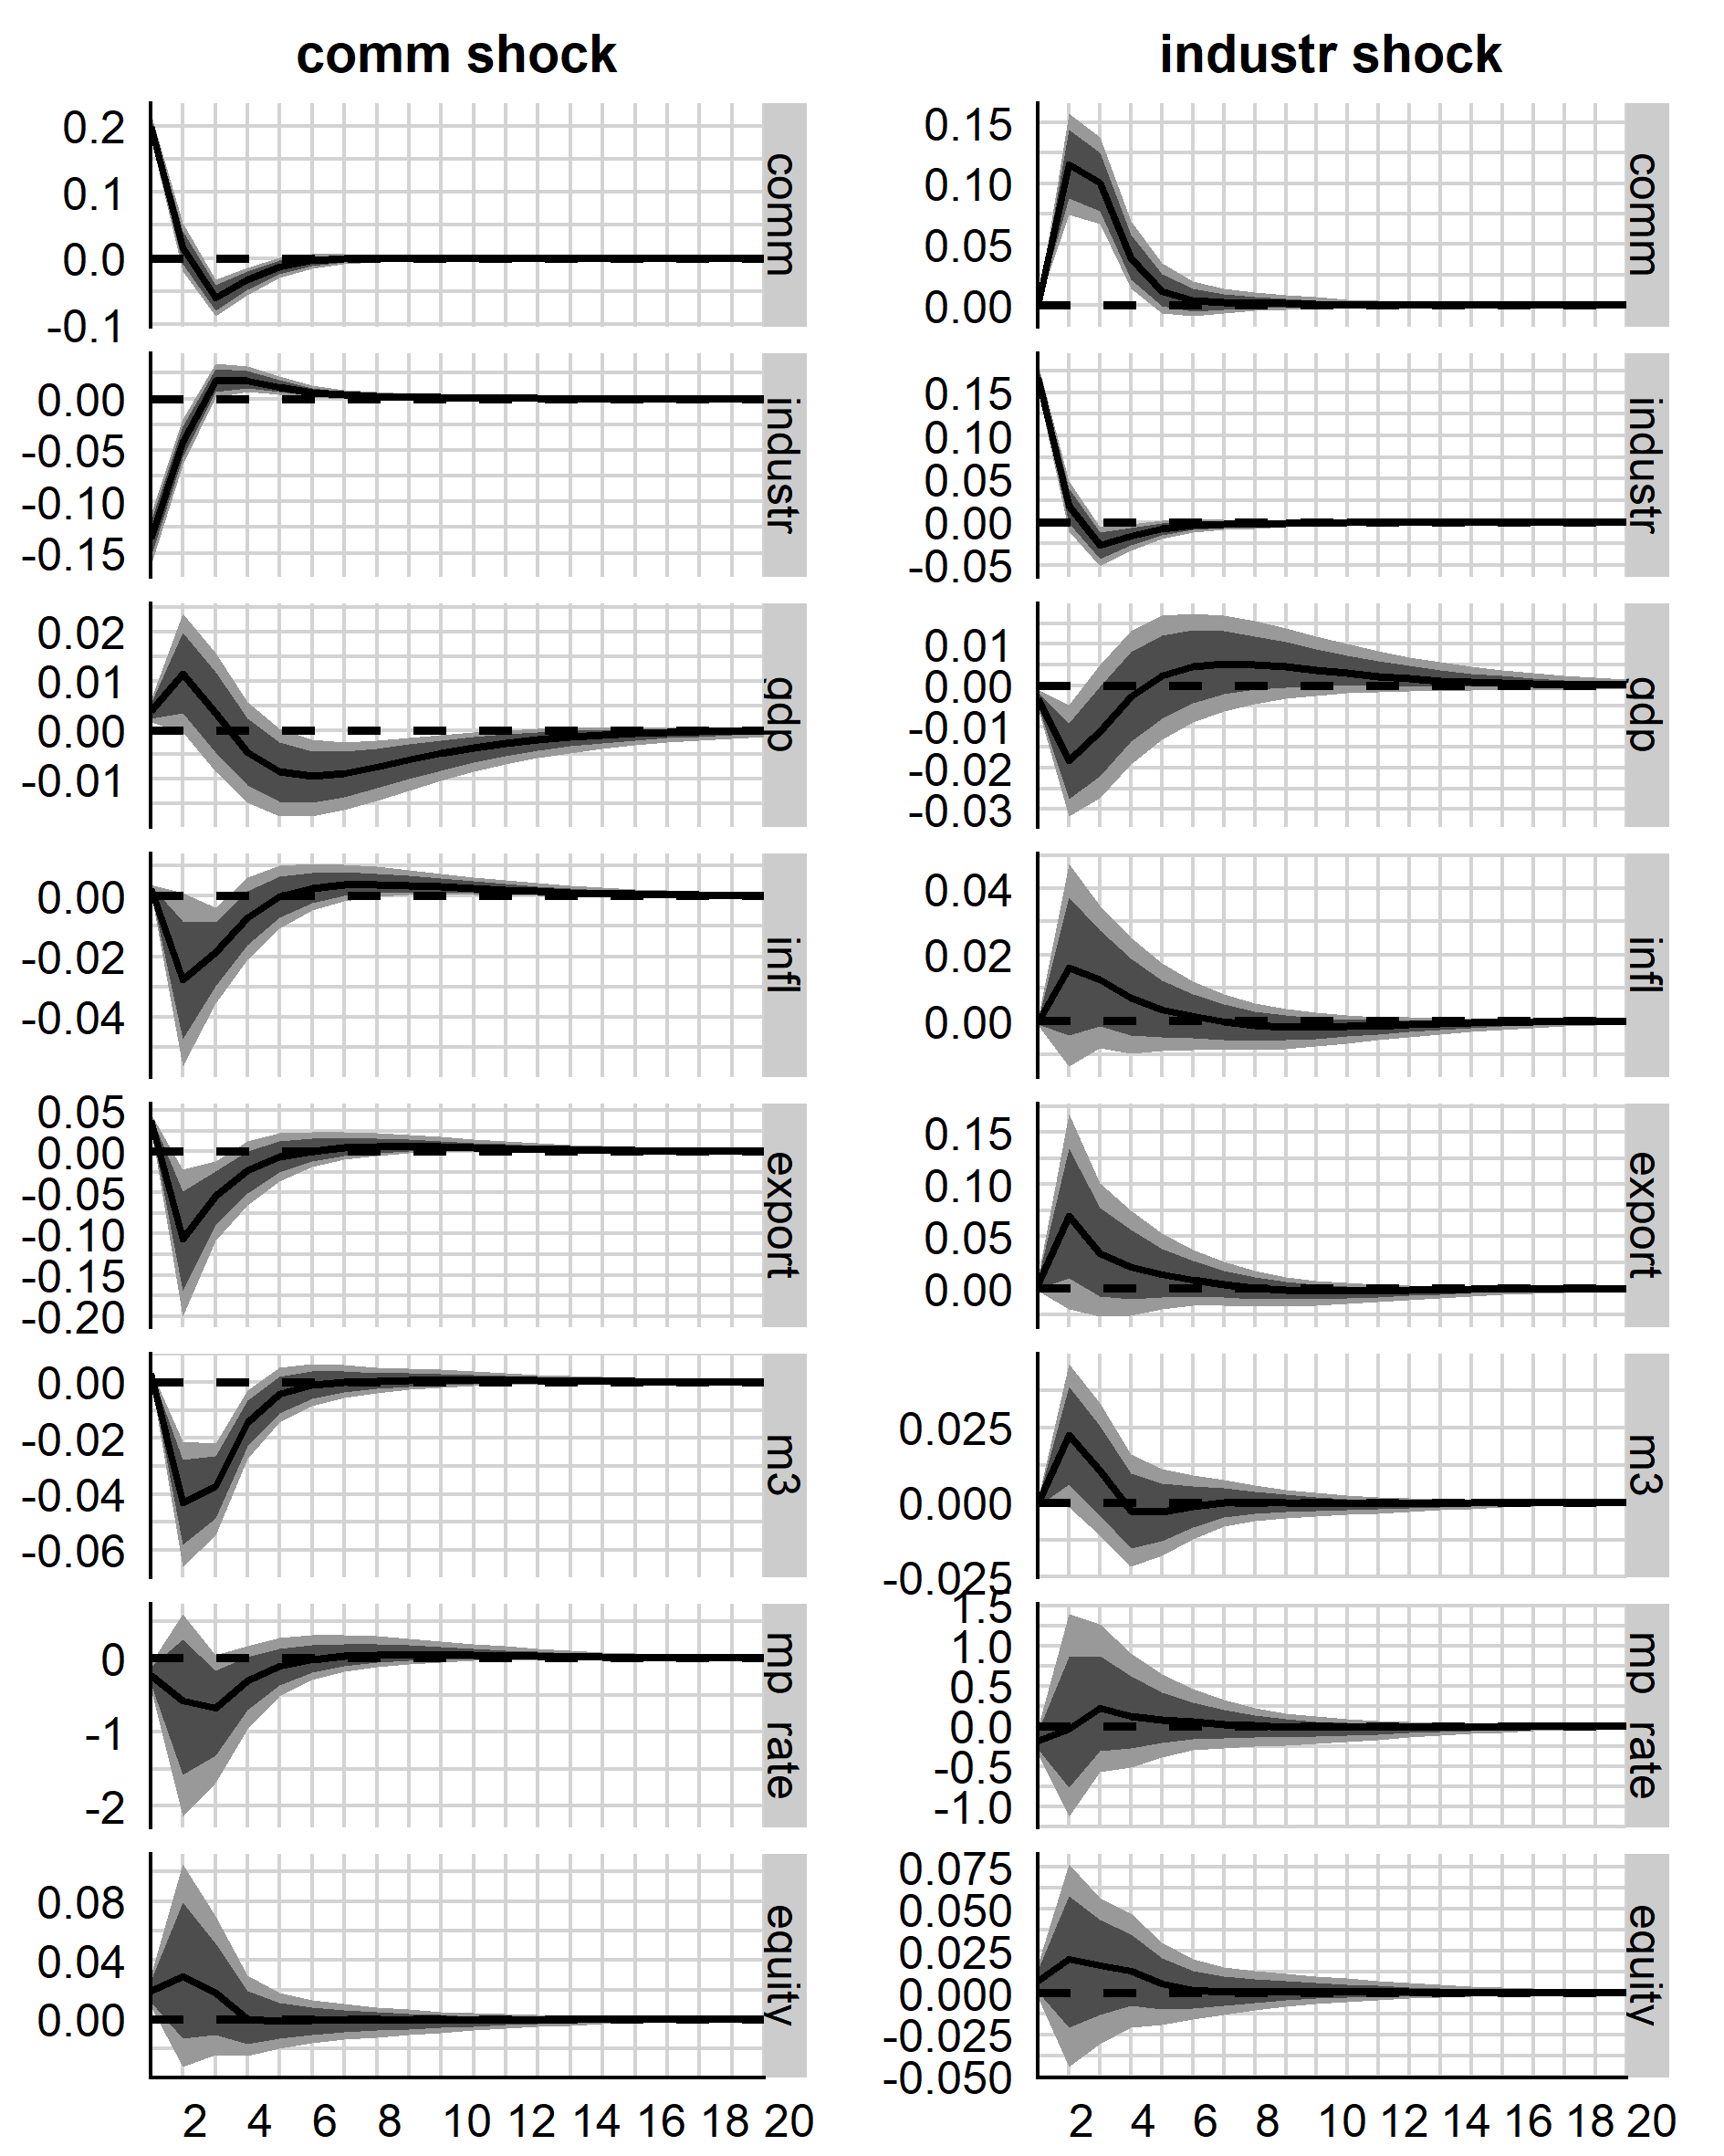
\includegraphics[width=0.50000\textwidth]{img/irf_short_CHL.png}
\caption{Impulse Responses, Chile}
\end{figure}

\begin{figure}
\centering
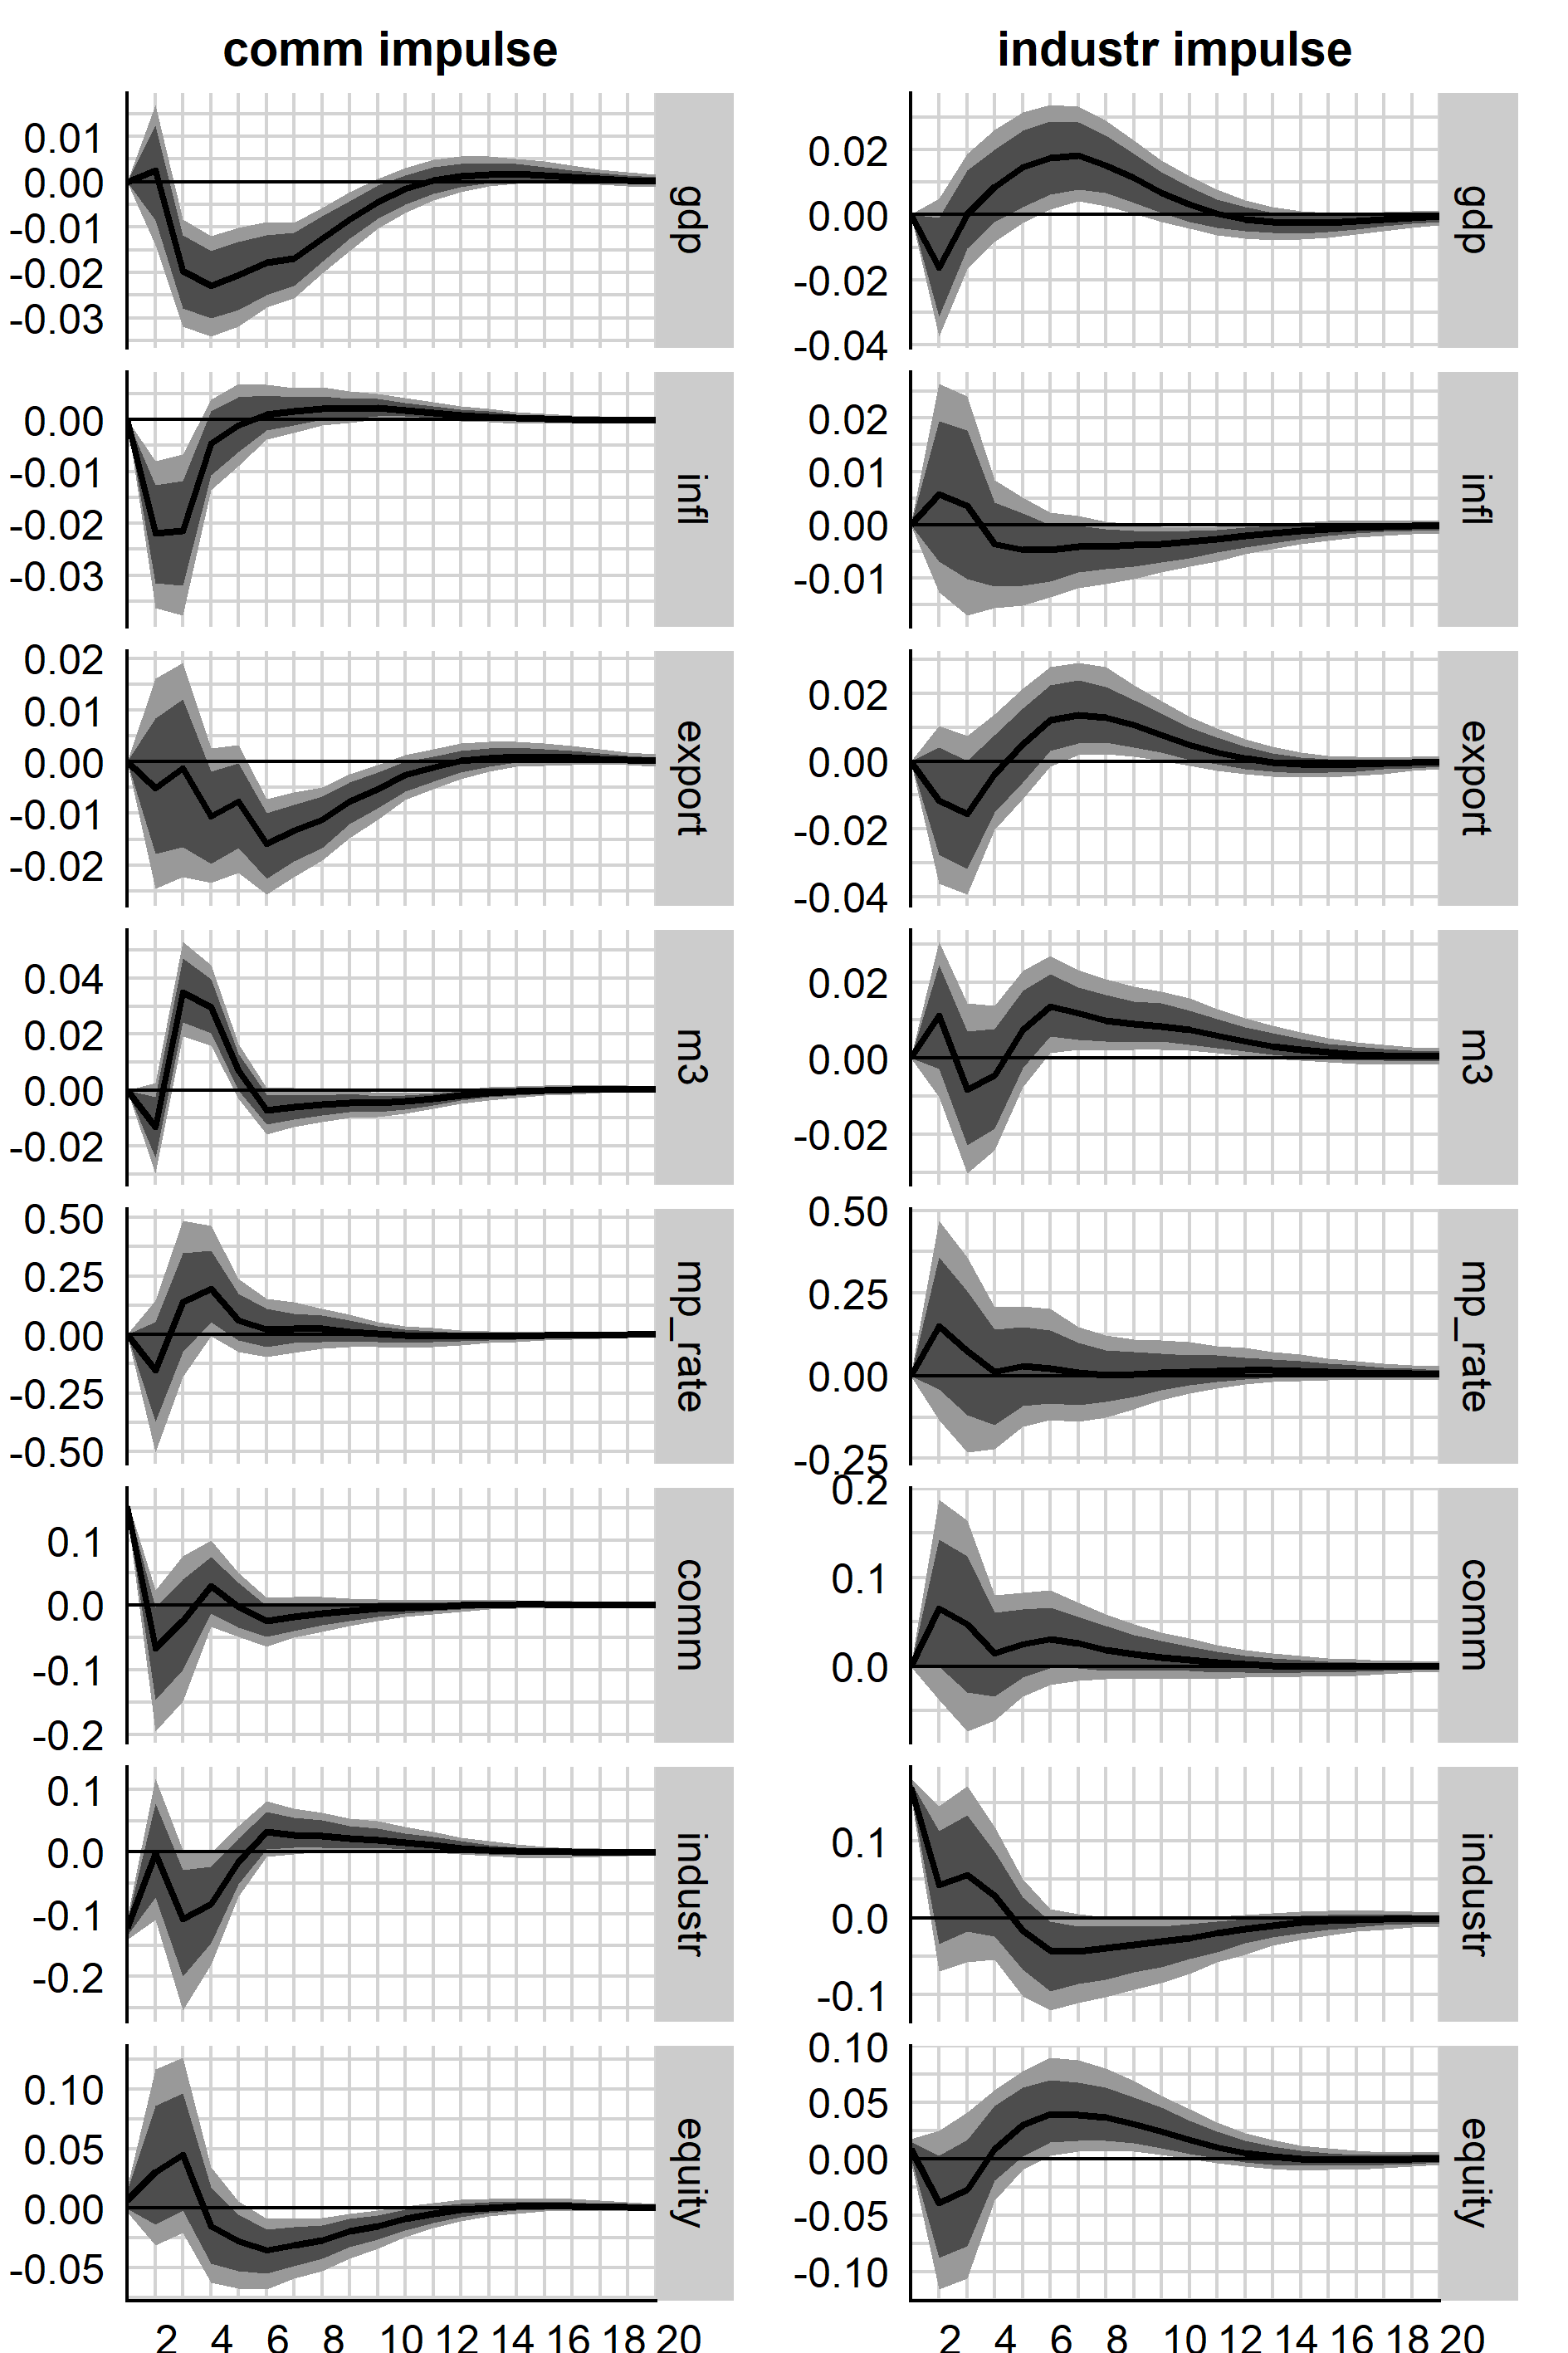
\includegraphics[width=0.50000\textwidth]{img/irf_short_NOR.png}
\caption{Impulse Responses, Norway}
\end{figure}

\begin{figure}
\centering
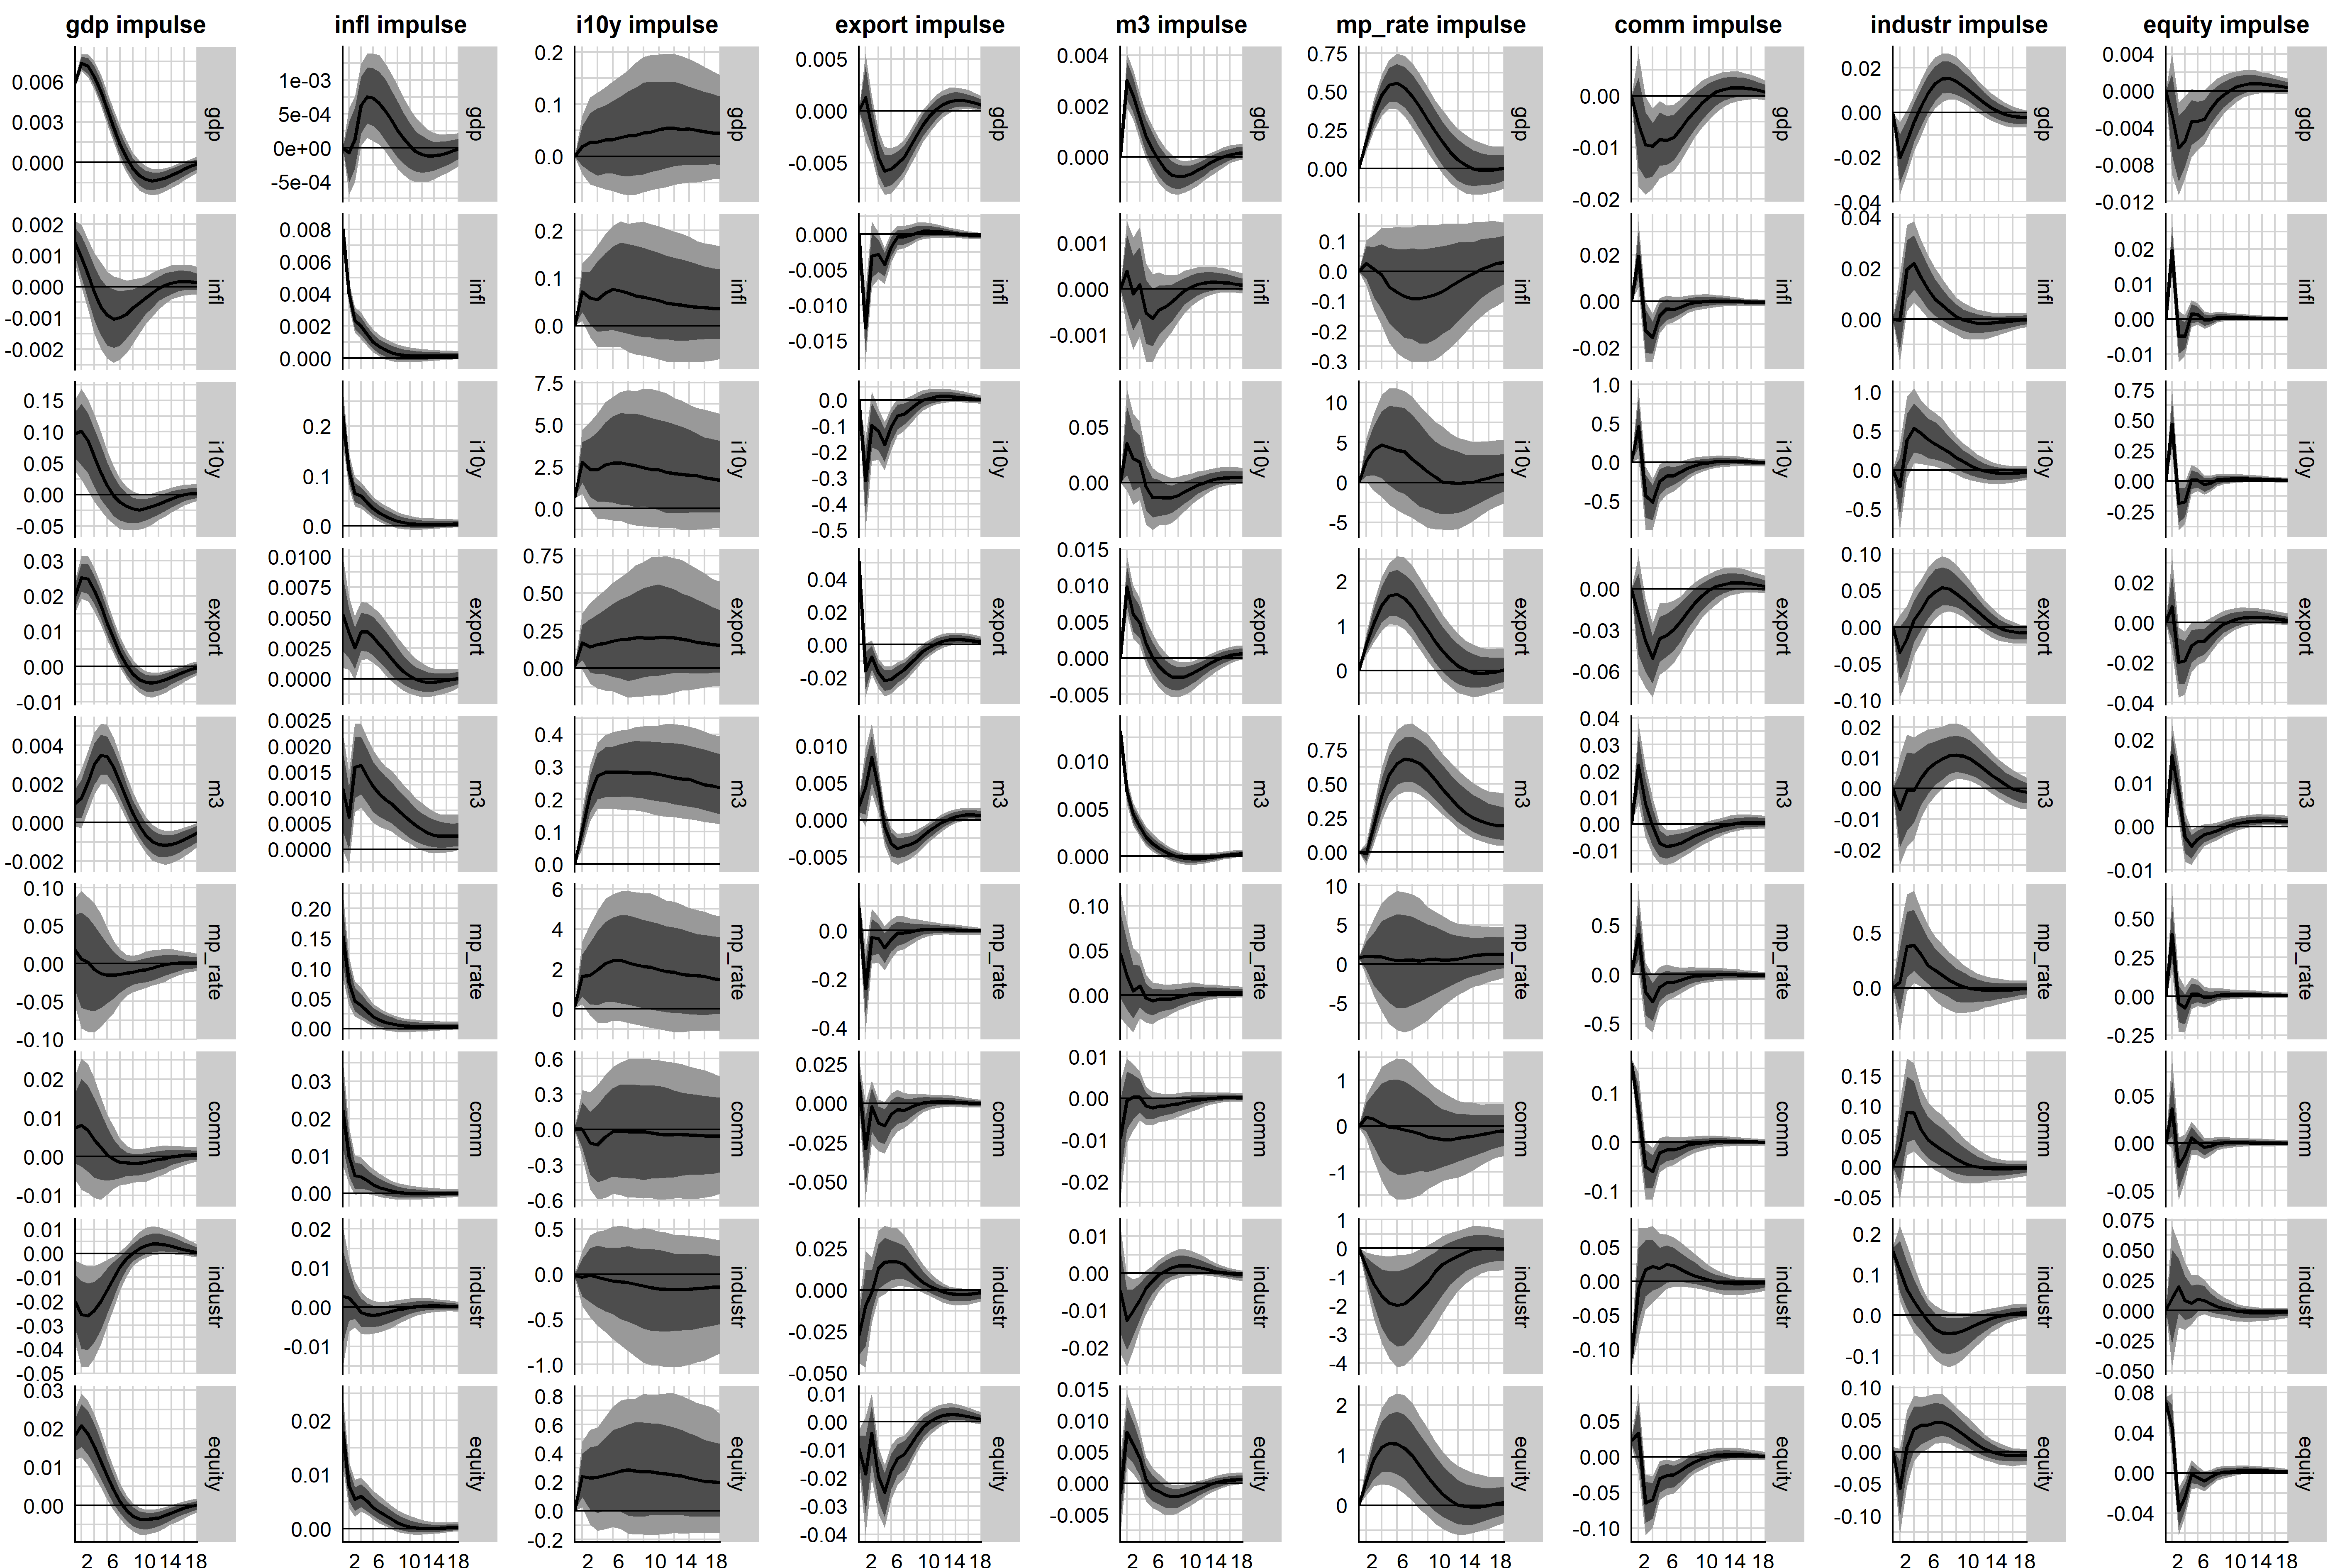
\includegraphics[width=1.00000\textwidth]{img/irf_all_ZAF.png}
\caption{Full Impulse Responses, South Africa}
\end{figure}

\begin{table}

\caption{\label{tab:unnamed-chunk-5}Selection of PC Analyses}
\centering
\begin{tabular}[t]{r|r|l|l|r}
\hline
Start & \# of Variables & Status & Bartlett's p & KMO Criterion\\
\hline
1970 & 11 & Rejected & < 2.22e-16 & 0.77\\
\hline
1975 & 12 & Rejected & < 2.22e-16 & 0.75\\
\hline
1980 & 14 & Accepted & < 2.22e-16 & 0.80\\
\hline
1985 & 16 & Rejected & < 2.22e-16 & 0.78\\
\hline
\end{tabular}
\end{table}

\begin{table}

\caption{\label{tab:unnamed-chunk-6}Variables in the PCA}
\centering
\begin{tabular}[t]{l|l|l}
\hline
Commodity Prices and Indices & Identifier & Source\\
\hline
Aluminium Index & NLSAH Index & Bloomberg\\
\hline
Copper Index & NLSCA Index & Bloomberg\\
\hline
Gold Price & XAG Curncy & Bloomberg\\
\hline
Lead Index & NLSPB Index & Bloomberg\\
\hline
Nickel Index & NLSNI Index & Bloomberg\\
\hline
Silver Price & XAU Curncy & Bloomberg\\
\hline
Zinc Index & NLSZS Index & Bloomberg\\
\hline
S\&P Gold Index & SPGSGC Index & Bloomberg\\
\hline
S\&P Commodity Index & SPGSCI Index & Bloomberg\\
\hline
S\&P Agriculture Index & SPGSAG Index & Bloomberg\\
\hline
S\&P Agriculture and Livestock Index & SPGSAL Index & Bloomberg\\
\hline
S\&P Livestock Index & SPGSLV Index & Bloomberg\\
\hline
S\&P Industrial Metals Index & SPGSIN Index & Bloomberg\\
\hline
\end{tabular}
\end{table}

\begin{table}

\caption{\label{tab:unnamed-chunk-7}Key figures of the PCA}
\centering
\begin{tabular}[t]{l|r|r}
\hline
Component & Component 1 & Component 2\\
\hline
SS loadings & 7.79 & 2.68\\
\hline
Proportion Variance & 0.60 & 0.21\\
\hline
Cumulative Variance & 0.60 & 0.81\\
\hline
Proportion Explained & 0.74 & 0.26\\
\hline
Cumulative Proportion & 0.74 & 1.00\\
\hline
\end{tabular}
\end{table}

\begin{figure}
\centering
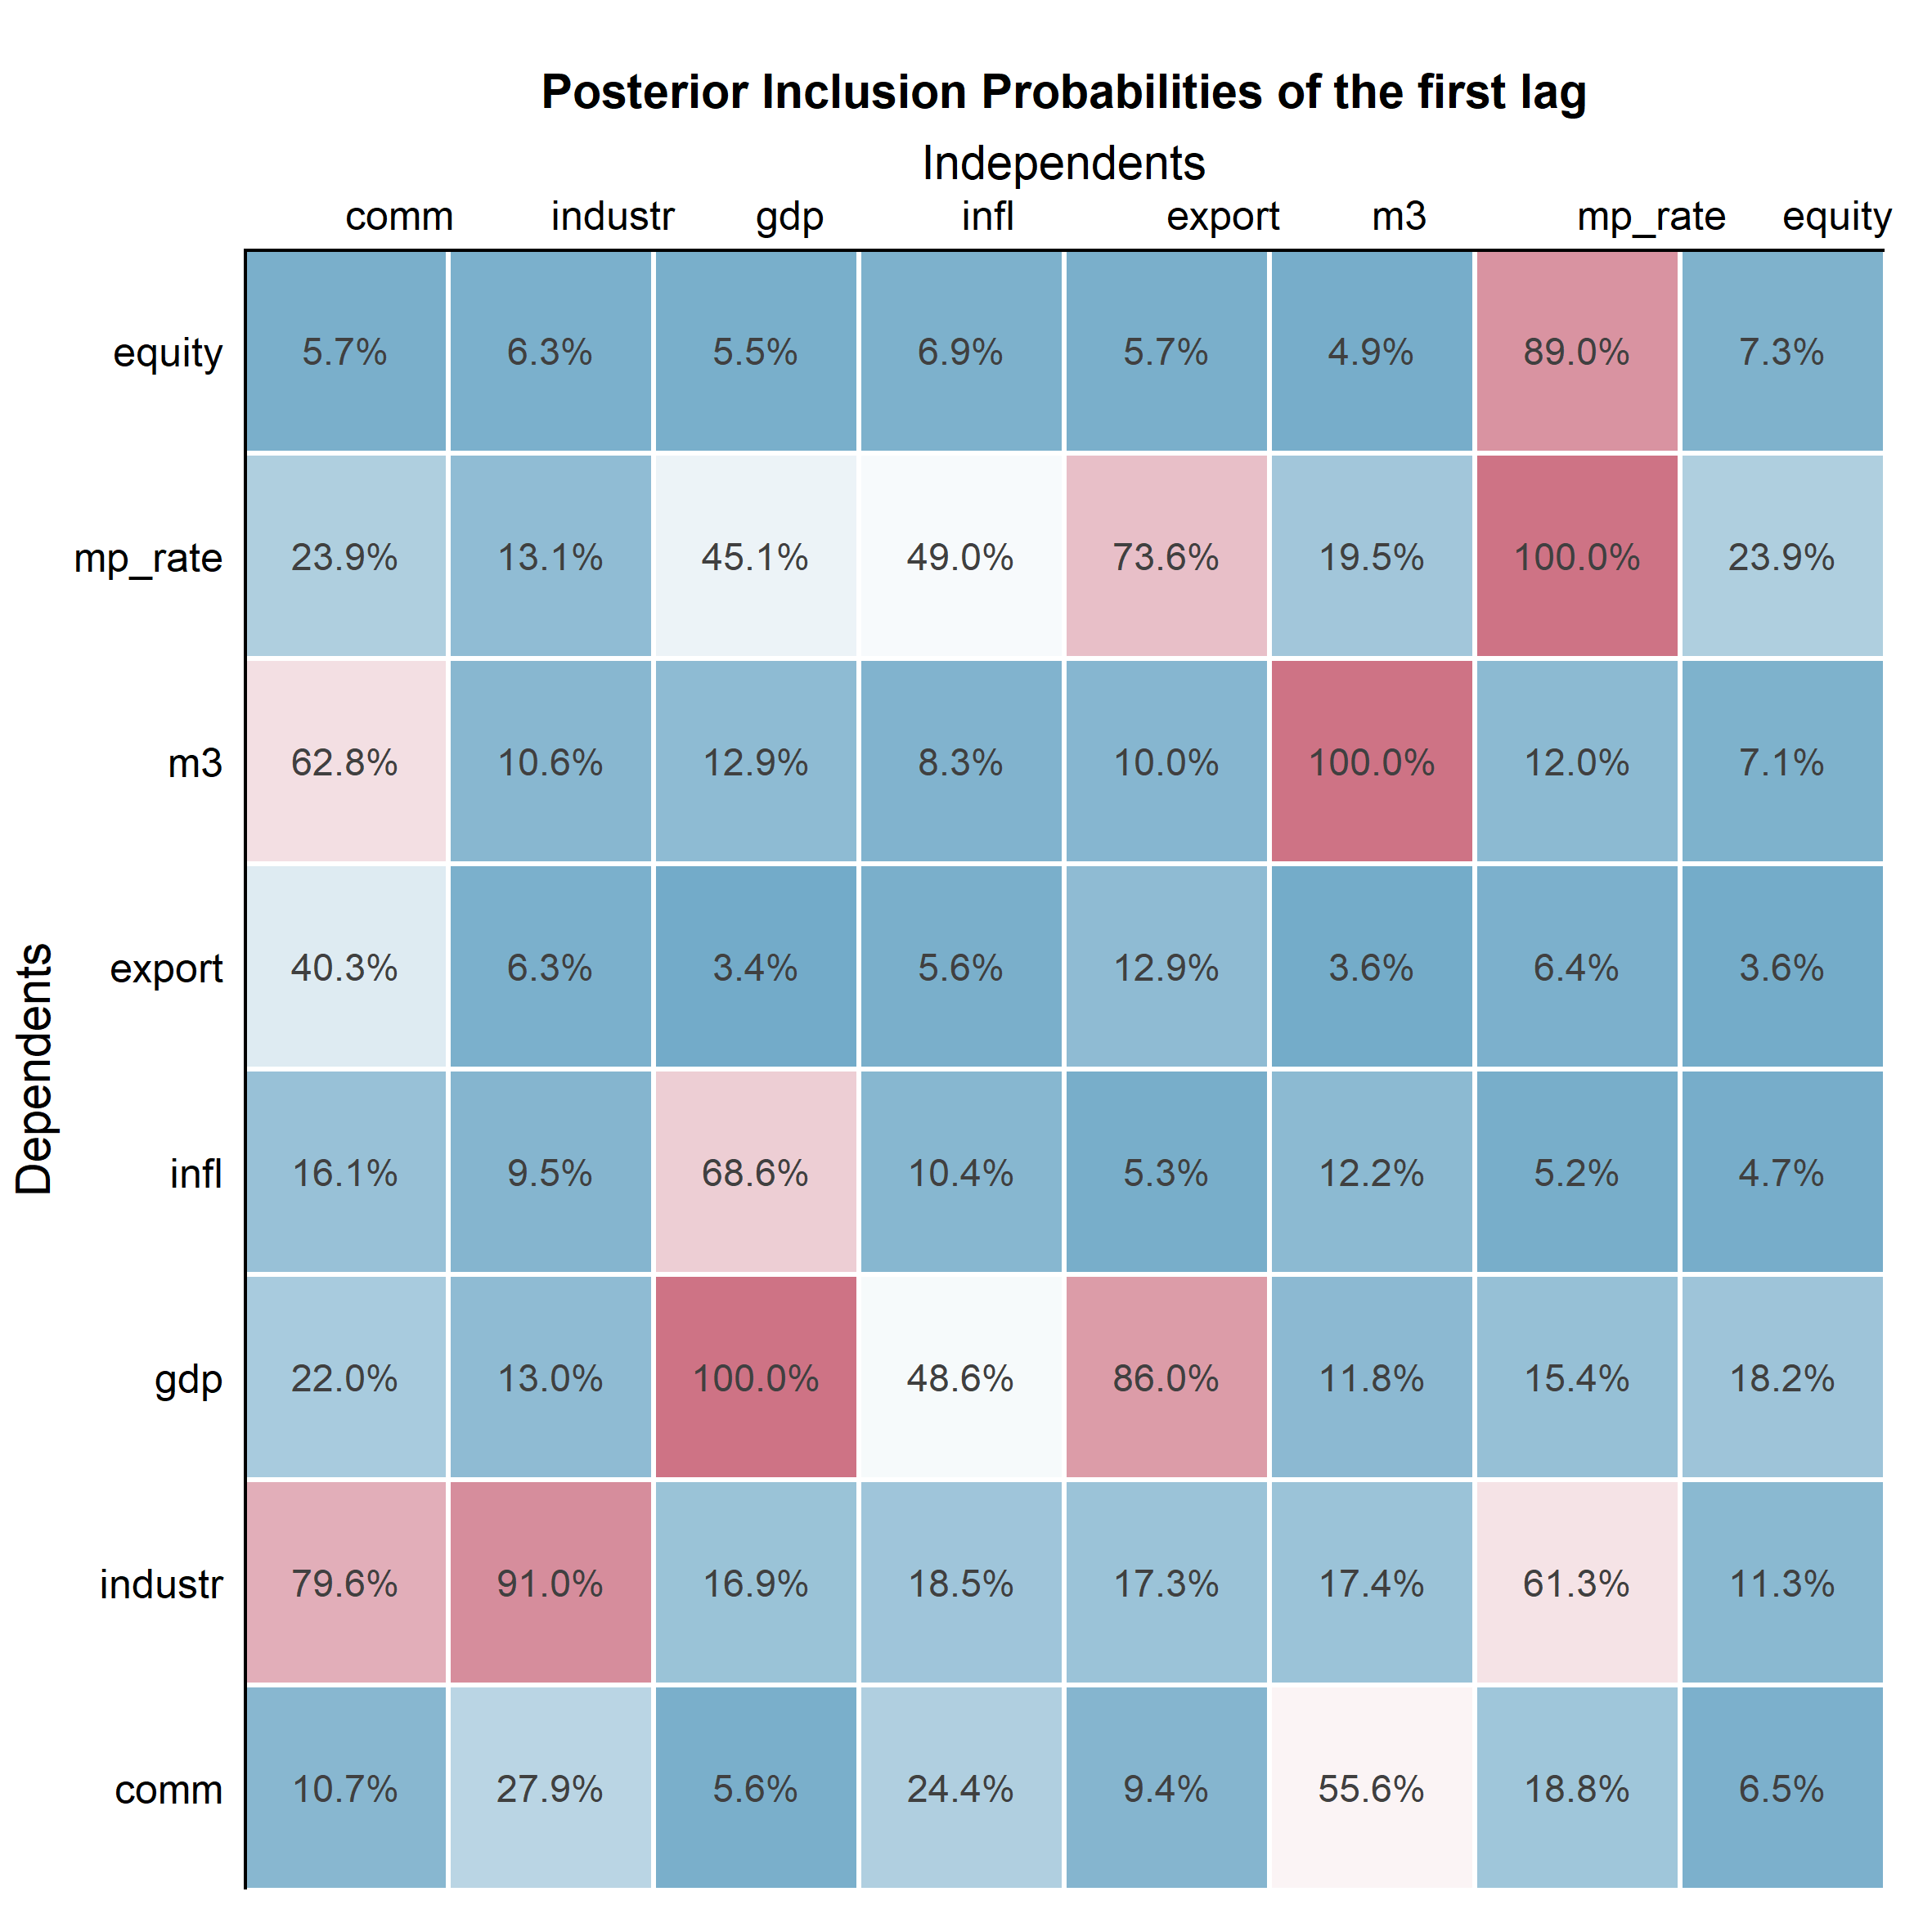
\includegraphics[width=0.50000\textwidth]{img/pip_heatmap_CHL.png}
\caption{Posterior Inclusion Probabilities, Chile}
\end{figure}

\begin{figure}
\centering
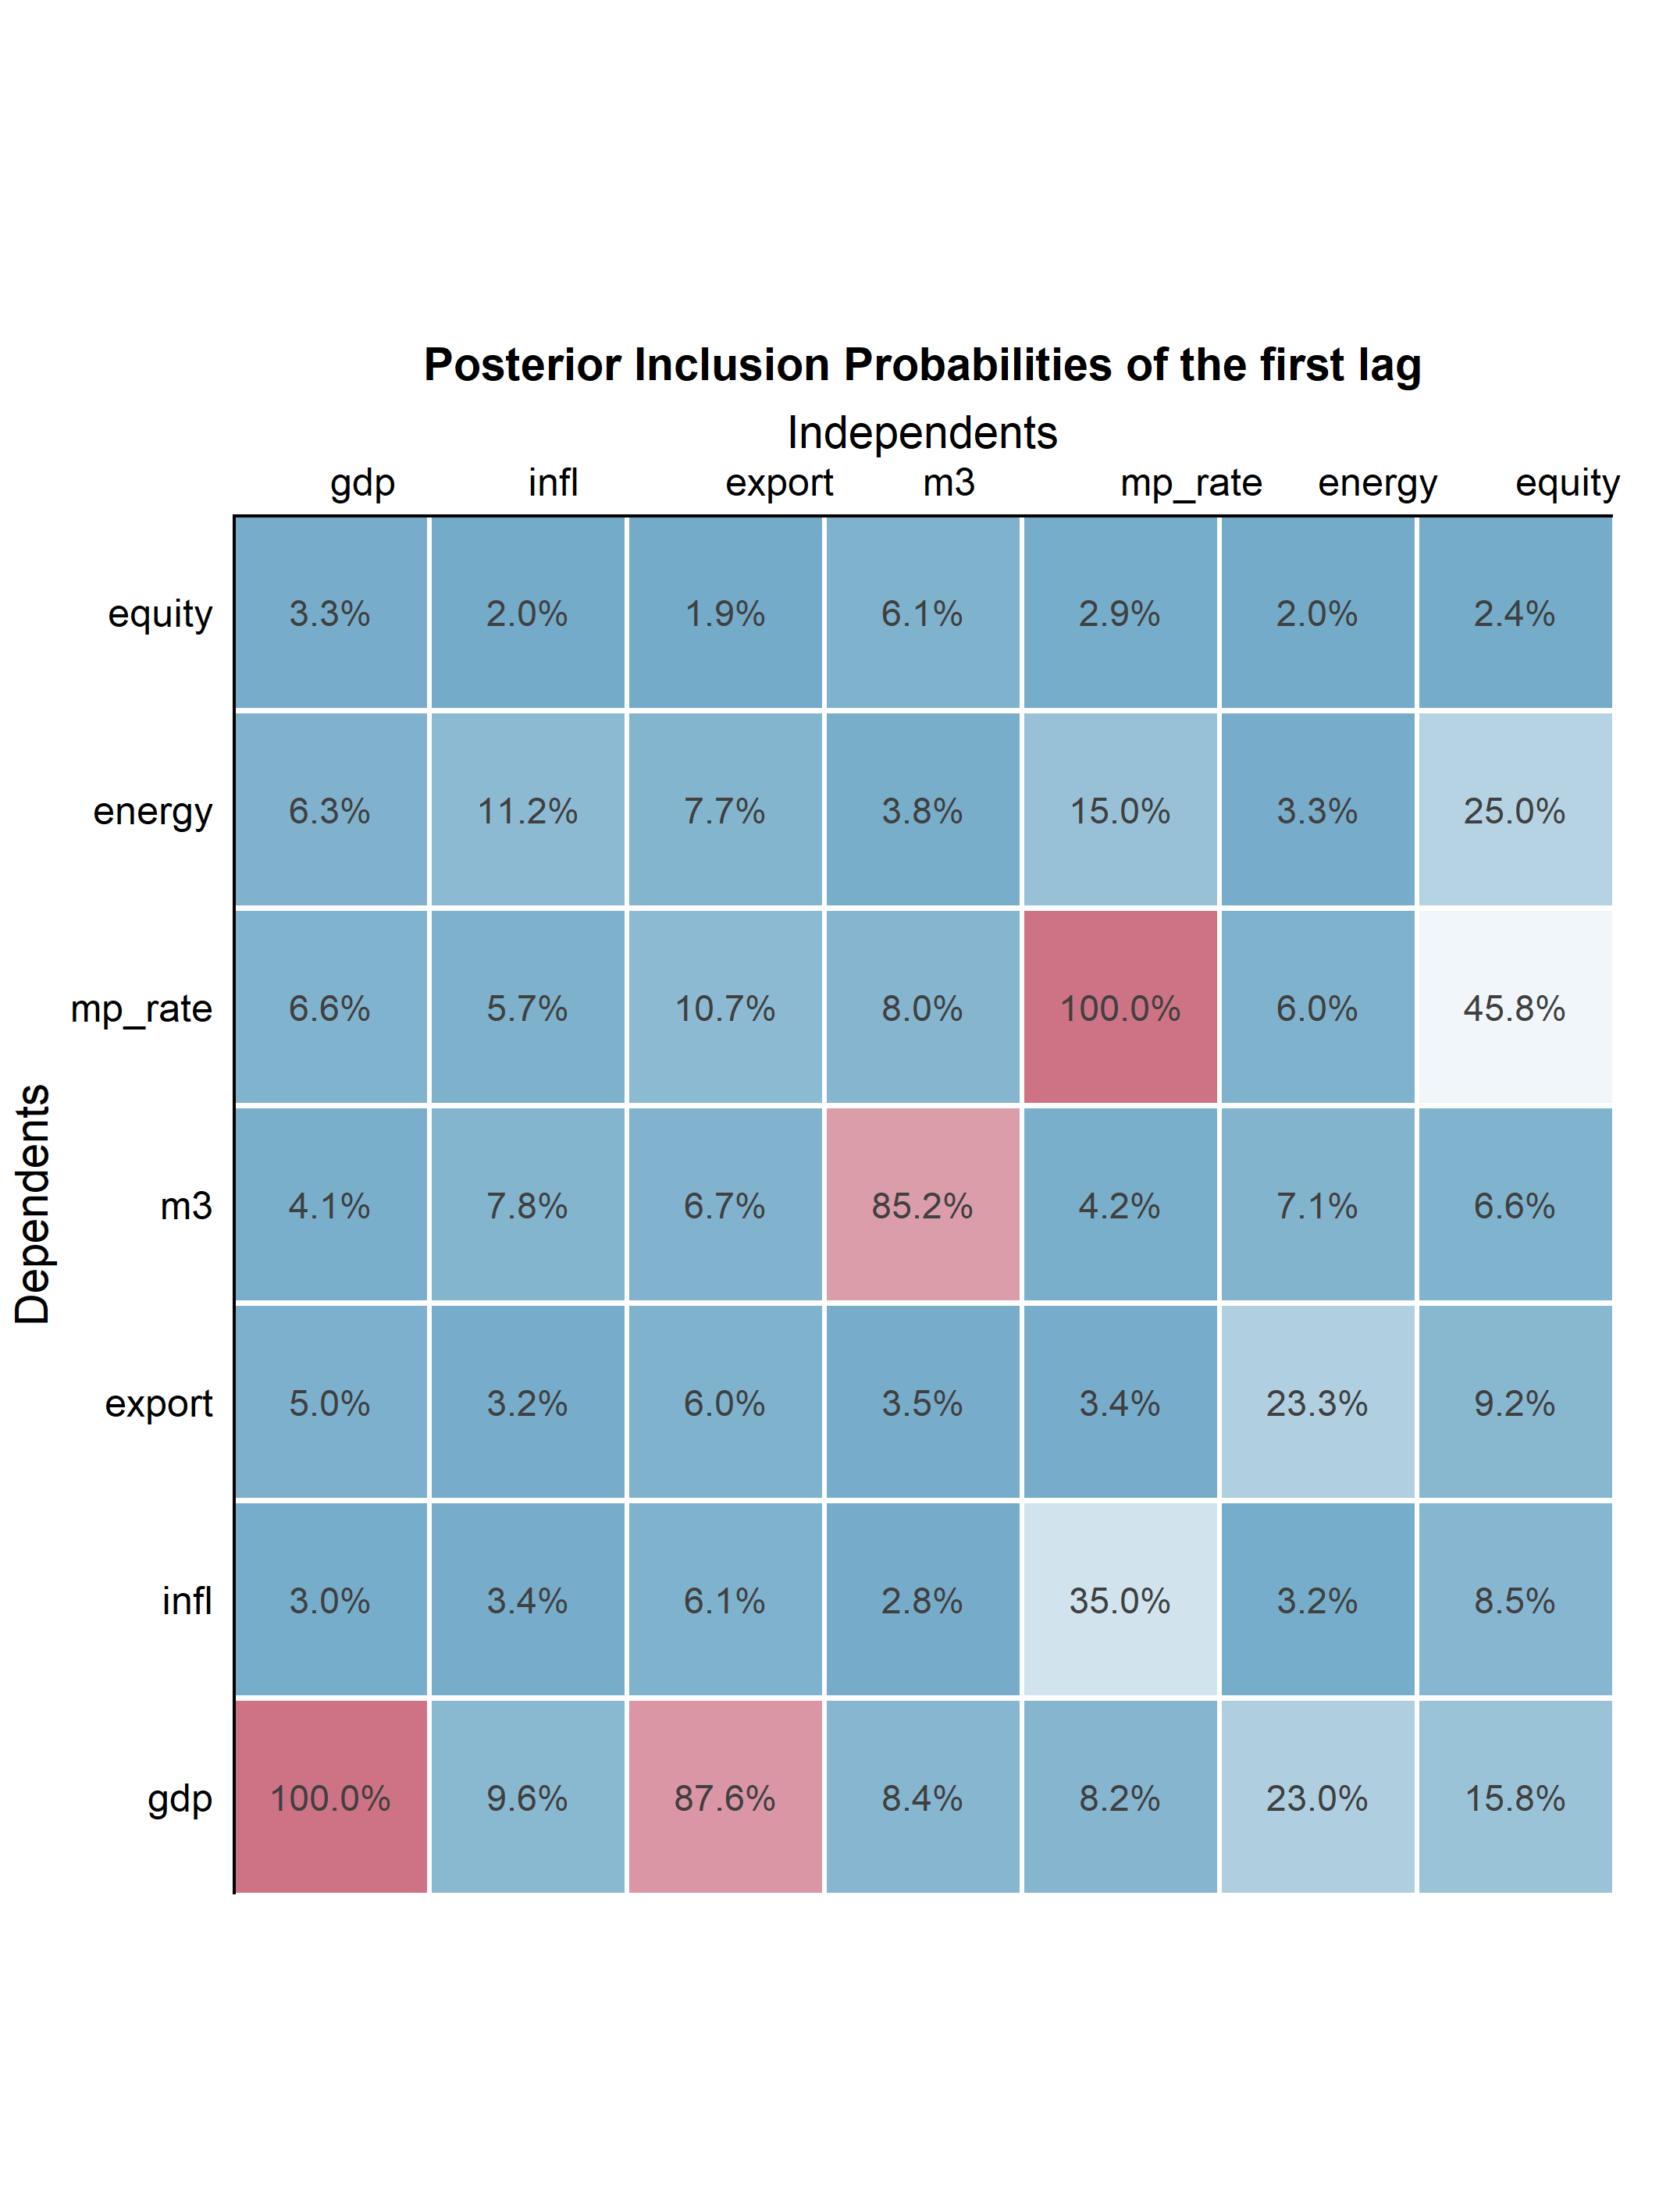
\includegraphics[width=0.50000\textwidth]{img/pip_heatmap_NOR.png}
\caption{Posterior Inclusion Probabilities, Norway}
\end{figure}


\end{document}
